\section{Implementierung Prototyp}
\label{sec:implementierung}

Nachdem im letzten Abschnitt eine Festlegung auf spezifischen Kriterien zur Erhebung von Messwerten vorgenommen wurde, folgt eine detaillierte Beschreibung der Implementierung des zu erstellenden Prototypen. Der komplette Quellcode sowie alle zugehörigen Konfigurationsdateien befinden sich in einem Github-Repository unter folgender Url \url{https://github.com/derMacon/stack-scale-benchmark} .

\subsection{Schichtenmodell \checkmark}
Der Arbeitsfluss der Anwendung wurde in Abbildung \ref{fig:stackOverview} visuell dargestellt. Die unterschiedlichen Komponenten wurden dabei in vier verschiedene Schichten eingeteilt: 

\begin{figure}[ht!]
	\centering
	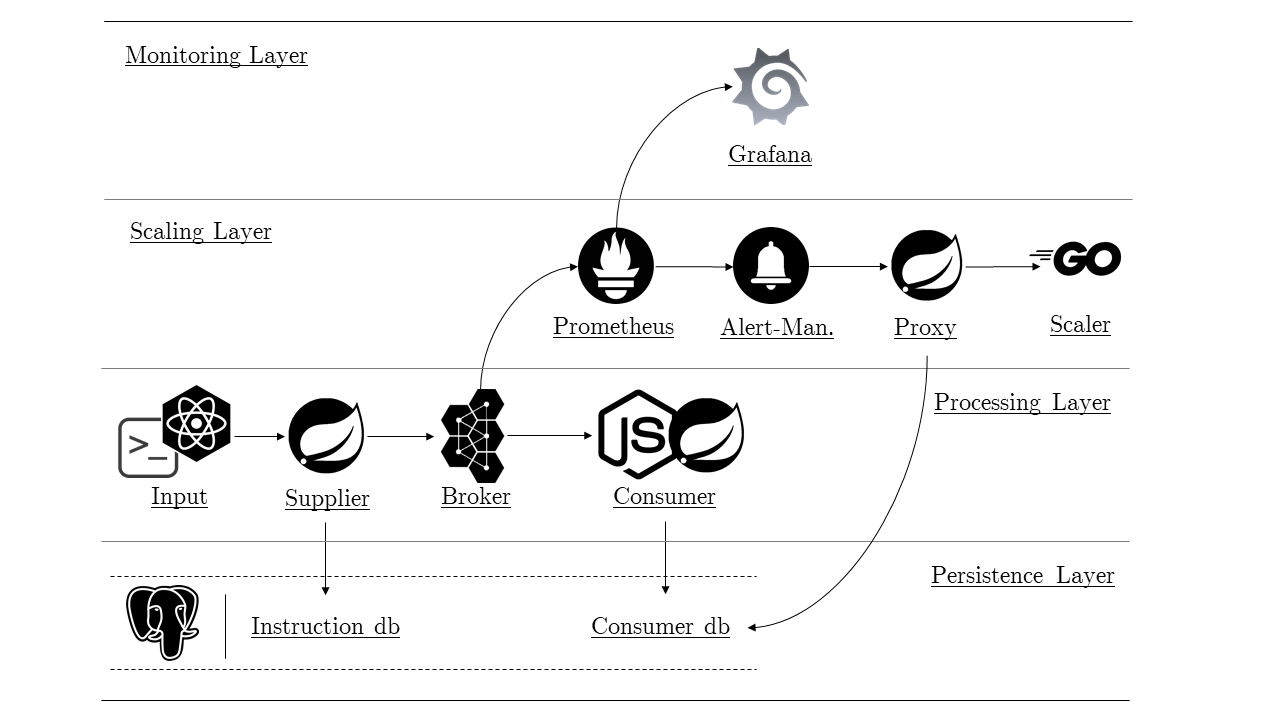
\includegraphics[width=\linewidth]{kapitel/problemloesung/implementierung/_img/overview-bw}
	\caption[Komponenten-Stack im Überblick]{Komponenten-Stack im Überblick}
	\label{fig:stackOverview}
\end{figure}

\begin{itemize}
  \item Persistenzschicht (engl. \emph{persistence layer}): Beinhaltet sämtliche Komponenten, die für das Abspeichern gegebener Datensätze in dazugehörige Datenbanken zuständig sind. Um Nebenläufigkeit zu ermöglichen wird hier ebenfalls auf Schnittstellen über einen Message-Broker zurückgegriffen. Eine Manipulation der Daten findet auf dieser Ebene nicht statt.
  \item Verarbeitungsschicht (engl. \emph{processing layer}): Beinhaltet sämtliche Komponenten, die für die direkte Verarbeitung der Business-Logik zuständig sind. Die Kommunikation zwischen den Komponenten findet über eine REST-Schnittstelle sowie einen Message-Broker statt. Der Message-Broker stellt hierbei vor allem eine nebenläufige Verarbeitung der konsumierenden Komponenten sicher. Allerdings bietet dieser ebenfalls die Schnittstelle zur Skalierungsschicht (engl. \emph{scaling layer}).
  \item Skalierungsschicht (engl. \emph{scaling layer}): Beinhaltet sämtliche Komponenten zum Skalieren der konsumierenden Komponenten. Hierbei wird auf eine universelle Schnittstelle des Message Broker zurückgegriffen um entsprechende Metriken abzugreifen, die für die Evaluierung hinterlegter Regeln zur Skalierung verwendet werden. Ansonsten wird in Komponenten dieser Schicht das Zeitverhalten des Initialisierungsprozesses der konsumierenden Komponenten überwacht und an Schnittstellen der Persistenzschicht weitergeleitet.
  \item Monitoring Ebene: Diese Schicht besteht aus einer einzigen Komponente, deren Aufgabe es ist erhaltene Daten visuell darzustellen. Um einen zeitlichen Überblick zu geben, werden die Daten intern vom Werkzeug gespeichert. Da es sich um lokal verwaltete Datensätze handelt, die für den Rest der Applikation keinerlei Bedeutung darstellen, wurde verzichtet eine Lösung zu finden, in der diese ebenfalls in einer Komponente der Persistenzschicht abzuspeichern.
\end{itemize}


\subsection{Komponenten im Überblick \checkmark}
Es folgt eine kurze Zusammenfassung der Funktionalität sowie der Anforderungen an die jeweilien Komponenten.

\subsubsection{Input \checkmark}
Um es dem Benutzer zu ermöglichen, gezielte Messwerte zu erfassen, wird eine REST-Schnittstelle vom System bereitgestellt. Es ist zwar möglich, dass der Benutzer selbstständig Anfragen für diese Schnittstelle generiert und absendet, beabsichtigt ist allerdings, dass der Benutzer auf vordefinierte Skripte oder eine entsprechende Benutzeroberfläche zurückgreift. Die Benutzeroberfläche ist sehr funktional gehalten, sodass es zwar möglich ist hierüber Anfragen an das System zu stellen, dennoch empfiehlt sich gerade für komplexere Anfrageszenarien der Gebrauch der bereitgestellten Bash-Skripte. Bezüglich der Skripte gibt es ebenfalls diverse Abstraktionsschichten. So ist es zum Beispiel möglich, mithilfe einer definierten Grammatik Anforderungen zu definieren, die sich beliebig kombinieren lassen. Hierzu wurden mehrere vordefinierte Dateien angelegt, deren Inhalt über ein entsprechendes Skript an das Backend geschickt werden können. Allerdings gibt es weitere Skripte, die auf diesem Prozess aufsetzen und somit eine Abstraktionsschicht aufbauen, sodass sich der Endbenutzer hiermit nicht auseinandersetzen muss. 


\subsubsection{Supplier \checkmark}
Diese Komponente ist in der Lage, die vereinfachten Anfragen des Benutzers zu interpretieren und in Nachrichten umzuwandeln, die vom System verarbeitet werden können. Hierbei werden bereits an dieser Stelle diverse Informationen an die ursprüngliche Nachricht angeheftet, um im späteren Verlauf entsprechende Metriken zu berechnen. Außerdem erfolgt eine erste Kommunikation mit der Persistenzschicht, in der die übersetzten Benutzeranfragen abgespeichert werden. Hierbei wird direkt auf die Datenbank zugegriffen, da im System lediglich eine Singleton-Instanz des \emph{Suppliers} vorhanden ist. Zwar unterstützt die verwendete Postgres-Datenbank mehrere Klienten zur gleichen Zeit, nativ ist diese Anzahl jedoch begrenzt und muss angemessen konfiguriert werden. Des Weiteren stellt die Supplier-Komponente zwei Modi hinsichtlich der Geschwindigkeit, in der Nachrichten an den Broker übermittelt werden. So ist es zum Beispiel möglich, Nachrichten über einen gewissen Zeitraum hinweg abzuschicken oder aber eine Transaktion zu bilden, in der alle auf einmal geschickt werden.


\subsubsection{Broker \checkmark}
Ein Message-Broker stellt die Funktionalität bereit, Nachrichten über ein gegebenes Protokoll an mehre Konsumenten zu vermitteln. Hierzu wurde eine Implementierung von Apache namens "\emph{Active MQ\footnote{\url{https://github.com/apache/activemq}}}" gewählt. Diese besitzt zwei Betriebsmodi, einmal das Arbeiten mit einer \emph{Topic} sowie mit einer \emph{Queue}. Eine Topic stellt ein \emph{Publisher-Subscriber-Muster} bereit, in dem alle eingehenden Nachrichten an alle registrierten Konsumenten verschickt werden \cite[Seite~33 ff.]{activemq-snyder}. Demgegenüber steht eine \emph{Queue} (Warteschlange), die eingehende Nachrichten lediglich an einen einzelnen Konsumenten übermittelt, wobei der Broker hierbei als eine Art Load Balancer\footnote{Erklärung \emph{Load Balancer} siehe Abschnitt \ref{sec:loadbalancer}} agiert. Bevor die Nachrichten jedoch aus einer der beiden Datenstrukturen entfernt werden, muss der betreffende Konsument eine \emph{Acknowledgement-Nachricht} an den Broker schicken, um zu signalisieren, dass die Nachricht nicht nur angenommen, sondern auch korrekt verarbeitet werden konnte. Es gilt ebenfalls noch hervorzuheben, dass die eingeschriebenen Konsumenten bei neuen Nachrichten stets benachrichtigt werden und es clientseitig keine Logik braucht, um zum Beispiel event- oder intervallbasiert eine Abfrage an den Broker zu steuern. Da diese Komponente ebenfalls den Einstiegspunkt für das Monitoring System \emph{Prometheus} (siehe Abschnitt \ref{ss:prometheus}) darstellt, benötigt der Broker eine Schnittstelle über die er diesem Tool Messdaten zur Verfügung stellen kann. Die von ActiveMq bereitgestellt Schnittstelle nennt sich "\emph{Java Management Extension API (JMX)}" und ist die Standard-API zur Verwaltung von Java Applikationen \cite[Seite~331 ff.]{activemq-snyder}.


\subsubsection{Consumer \checkmark}
Die konsumierenden Komponenten können beliebig skaliert werden und implementieren die in Abschnitt \ref{ss:fiktiverWorkflow} definierten Arbeitsschritte. Hierbei wird auf diverse Libraries zurückgegriffen, wobei die restliche Logik eher schlicht gehalten wurde. Die Komponenten kommunizieren lediglich über den Message-Broker mit dem Nachrichten-Supplier und über einen weiteren Nachrichten-Broker mit der Persistenzschicht um die extrahierten Elemente abzulegen.


\subsubsection{Prometheus \checkmark}
\label{ss:prometheus}
"\emph{Prometheus is an open source systems monitoring and alerting toolkit}" \cite[Seite~400]{oreillyPrometheus}. Es ist möglich über eine definierte Anfragensprache Daten Dritter zu verarbeiten. Diese Daten können über ein einfaches Textformat von den Komponenten ausgegeben werden. Es ist möglich dieses Textformat händisch zu schreiben, allerdings wird in der Praxis vermehrt auf Libraries, die auf den Client zugeschnitten wurden, gesetzt. Prometheus ist unter der Apache 2.0 Lizenz veröffentlicht \footnote{https://github.com/prometheus/prometheus}, und wurde primär in der Programmiersprache Go implementiert. Das intervallbasierte Anfragen (engl. "\emph{scrapen}") der Metriken wird von der Prometheus-Komponente selbst durchgeführt, die zu überwachenden Komponenten müssen sich selbst nicht darum kümmern Daten an Prometheus zu übermitteln.

\todo{checken ob Figure am Ende immer noch nicht unter die folgenden Absatz auf Seite passt, ggf. aendern}
\begin{figure}[ht!]
	\centering
	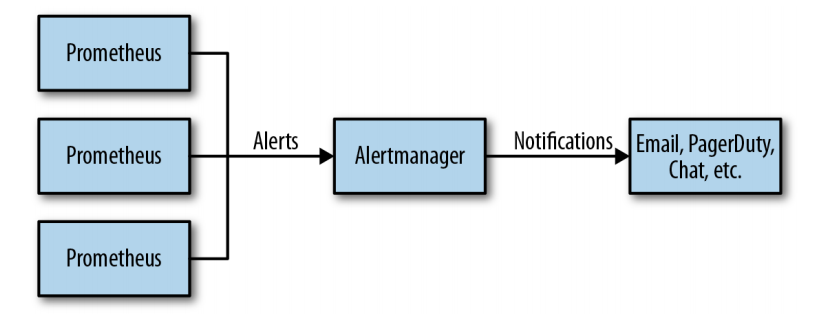
\includegraphics[width=.8\linewidth]{kapitel/problemloesung/implementierung/_img/alert-man-p291}
	\caption[Alert Manager - Übersicht]{Alert Manager - Übersicht \cite[Seite~291]{oreillyPrometheus}}
	\label{fig:alertManOverview}
\end{figure}

\subsubsection{Alert Manager \checkmark}
"\emph{Alerting is one of the components of monitoring, allowing you to notify a human when there is a problem}" \cite[Seite~291]{oreillyPrometheus}. Prometheus bietet hierbei die Möglichkeit mithilfe der funktionalen Anfragesprache \emph{PromQl} diverse Bedingungen zu definieren unter denen dies geschehen soll. Da es in einer produktiven Containerumgebung durchaus möglich ist, dass mehrere Prometheus-Instanzen parallel arbeiten, wurde das Benachrichtigen in eine weitere Komponente (den \emph{Alert Manger}) ausgelagert. Dieser synchronisiert, sammelt und gruppiert die Alerts der verschiedenen Prometheus-Instanzen und sendet Benachrichtigungen an definierte Nachrichtenkanäle, die sich beispielsweise aus einem Emailpostfach, einer Pagernachricht oder Chatnachricht auf Plattformen wie Slack zusammensetzen können (siehe Abbildung \ref{fig:alertManOverview}).


\subsubsection{Scaler Proxy \checkmark}
Diese Komponente bietet eine REST-Schnittstelle, die im Alert-Manager hinterlegt wird. Sobald eine der Regeln anschlägt, wird der Aufruf an diese Komponente weitergeleitet. Im Endeffekt dient diese Komponente lediglich als Proxy-Service, da ihre primäre Aufgabe darin besteht diese Nachricht an eine weitere Komponente weiterzuleitet. In einer produktiven Umgebung würde diese Komponente komplett enfallen, da es möglich ist den Alert-Manager derartig zu konfigurieren, dass er direkt die öffentlichen Schnittstellen der Scaler-API anspricht. Es wurde sich dennoch für das Zwischenschalten eines solchen Proxy-Services entschieden um genauere Messwerte zu erhalten. Gerade hinsichtlich der Initialisierungsphasen von Containern ist es angebracht so kurz vorher wie möglich einen Timestamp zu setzen. Da es keine Möglichkeit gibt direkt in die Konfiguration der Scaler-Api einzugreifen ist diese Lösung der nächstbeste Ansatz. Sobald eine Skalierungsanfrage weitergeleitet wurde, wird diese noch unbeantwortete Anfrage intern in einer Datenstruktur abgelegt. Sobald ein entsprechender Container komplett initialisiert wurde, ruft dieser eine weitere Schnittstelle des Proxy-Services auf. Daraufhin wird ein \emph{Acknowledgement-Timestamp} in der hinterlegten Anfrage gesetzt und an die Persistenzschicht weitergeleitet. 

Außerdem bietet diese Komponente die Möglichkeit für den Benutzer direkt Exemplare eines Consumers hochzufahren. Die verwendete Schnittstelle dient als Umgehung des herkömmlichen Programmflusses und wird zur Generierung der skalierungsschichtenunabhängigen Metrikberechnung verwendet (siehe Abschnitt \ref{par:specContainer}). Über dedizierte Endpunkte können diese Metriken als .csv Datei ausgelesen werden. 


\subsubsection{Scaler \checkmark}
"\emph{The goal of the Docker Scaler project is to provide a REST HTTP interface to scale services and nodes}"\cite{docker-scaler}. Außerdem werden mit jeder Skalierungsanfrage Statusinformationen über die aktuelle sowie zukünftige Anzahl von Instanzen des zu skalierenden Services zurückgegeben, die es dem Proxy-Service ermöglichen davon ausgehend einen Skalierungsstop für neue Anfragen beizubehalten oder aufzuheben. Dieser ist nötig damit das System keine weiteren Skalierungsprozesse starten, wenn bereits aktive Skalierungen vorgenommen werden.


\subsubsection{Grafana \checkmark}
Wenn es zum Alert durch den Alert Manager kommt, wird in einer Produktivumgebung der Erste Schritt sein die Performanz des Systems durch dedizierte Dashboard zu überprüfen \cite[Seite~97]{oreillyPrometheus}. Grafana ist ein Werkzeug, das dies über eine Weboberfläche direkt im Browser ermöglicht. Es bietet die Möglichkeit Graphen, Tabellen und weitere Visualisierungskomponenten zu erstellen um zum Beispiel die Latenzzeit oder CPU Auslastung zu überprüfen. Diese Metriken können für das ganze System oder nur einen Teil generiert werden. Es ist das bevorzugte Visualisierungswerkzeug für Prometheus, bietet allerdings ebenfalls Unterstützung für verschiedene weitere Systeme wie zum Beispiel \emph{Graphite}, \emph{Elasticsearch} oder \emph{PostgreSQL}.


\subsubsection{Mock scaler api \checkmark}
Diese Komponente ist nicht Kernbestandteil des Komponenten-Stacks. Sie dient lediglich während der Entwicklungszeit dazu die Scaler-Api zu emulieren. So ist es zum Beispiel möglich lokal eine Instanz des Scaler-Proxy Projekts in einer beliebigen IDE als Standard Spring Projekt auszuführen. Sämtliche Skalierungs-Anfragen können von dieser Komponente angenommen werden, da sie auf dem gleichen Port wie der "\emph{echte}" Scaler läuft, wobei sie dabei ebenfalls in der Lage ist diverse Rückgabenachrichten an den Klienten zu übergeben.


% \begin{figure}
% 	\centering
% 	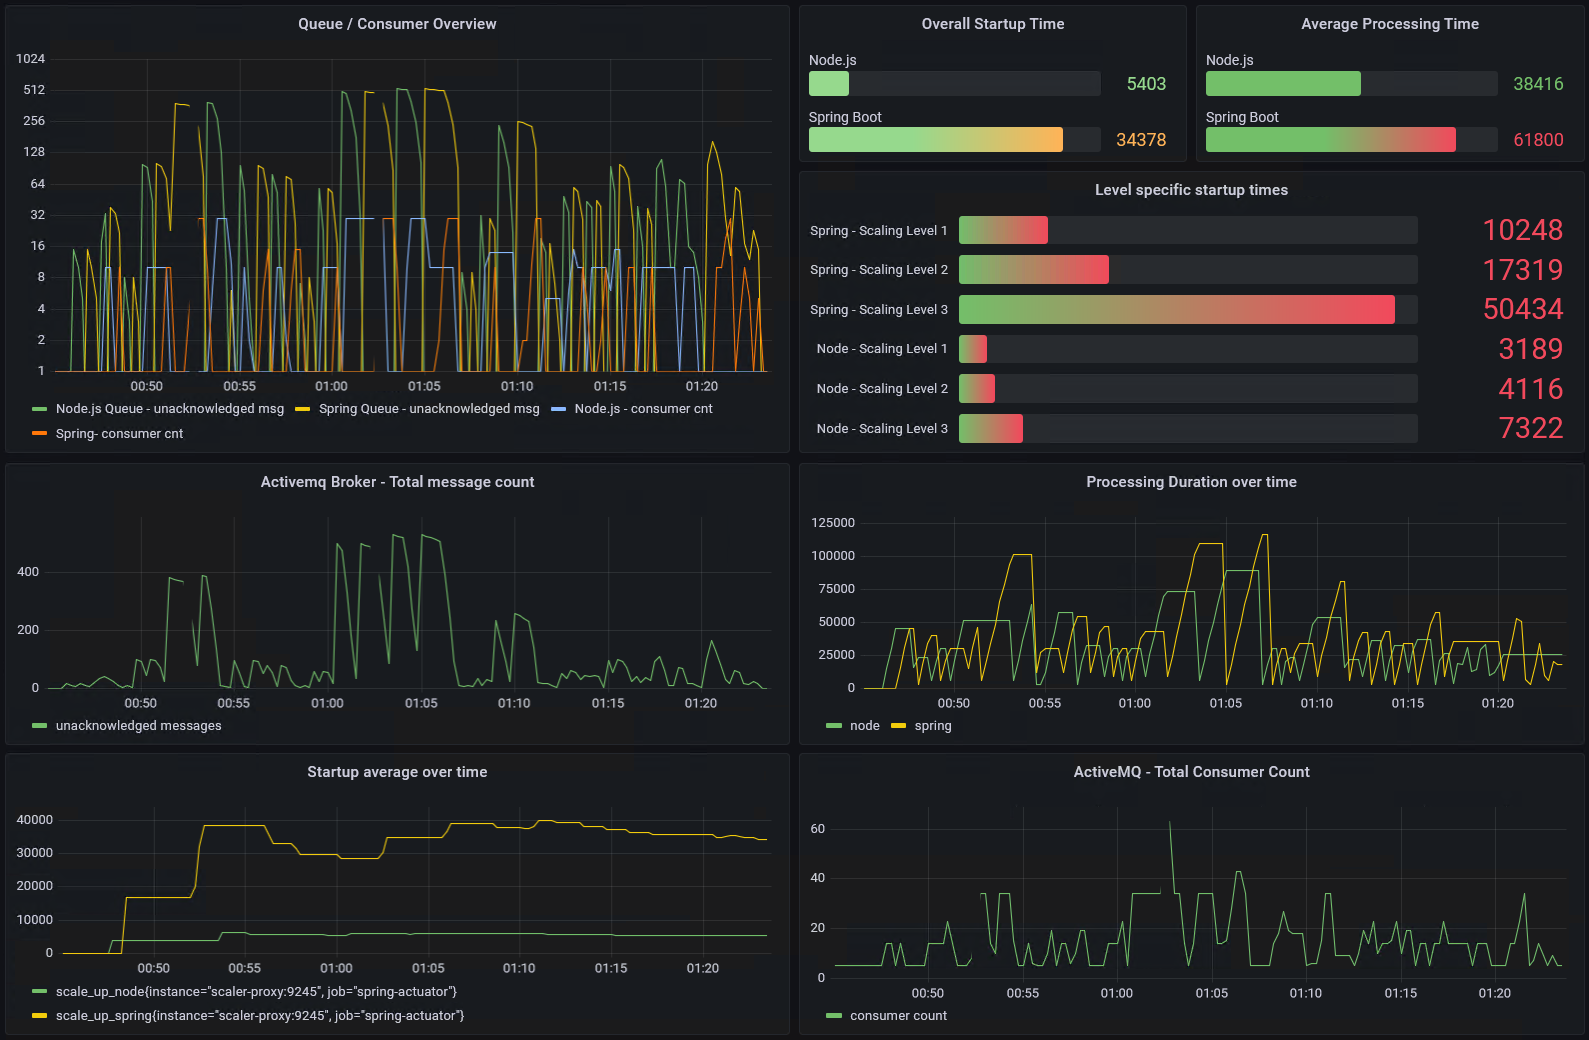
\includegraphics[width=\linewidth]{kapitel/problemloesung/implementierung/_img/grafana-dashboard-01}
% 	\caption[]{Grafana Dashboard}
% 	\label{fig:grafanaOverview}
% \end{figure}


\subsection{Input \checkmark}

Der Benutzer besitzt die Möglichkeit, sowohl über eine Benutzeroberfläche als auch über Bash-Skripte Benchmark Anfragen an das System zu stellen. Im Folgenden wird beides im Detail erläutert.

\subsubsection{Bash \checkmark}
\paragraph{Aufbau}
In der folgenden Abbildung ist der Aufbau des Bash-Projektes dargestellt. Der Benutzer besitzt drei Möglichkeiten Anfragen an das System zu stellen. Für jeden  Einstiegspunkt wurde ein entsprechendes Bash-Skript zur Verfügung gestellt

\begin{figure}[ht!]
	\centering
	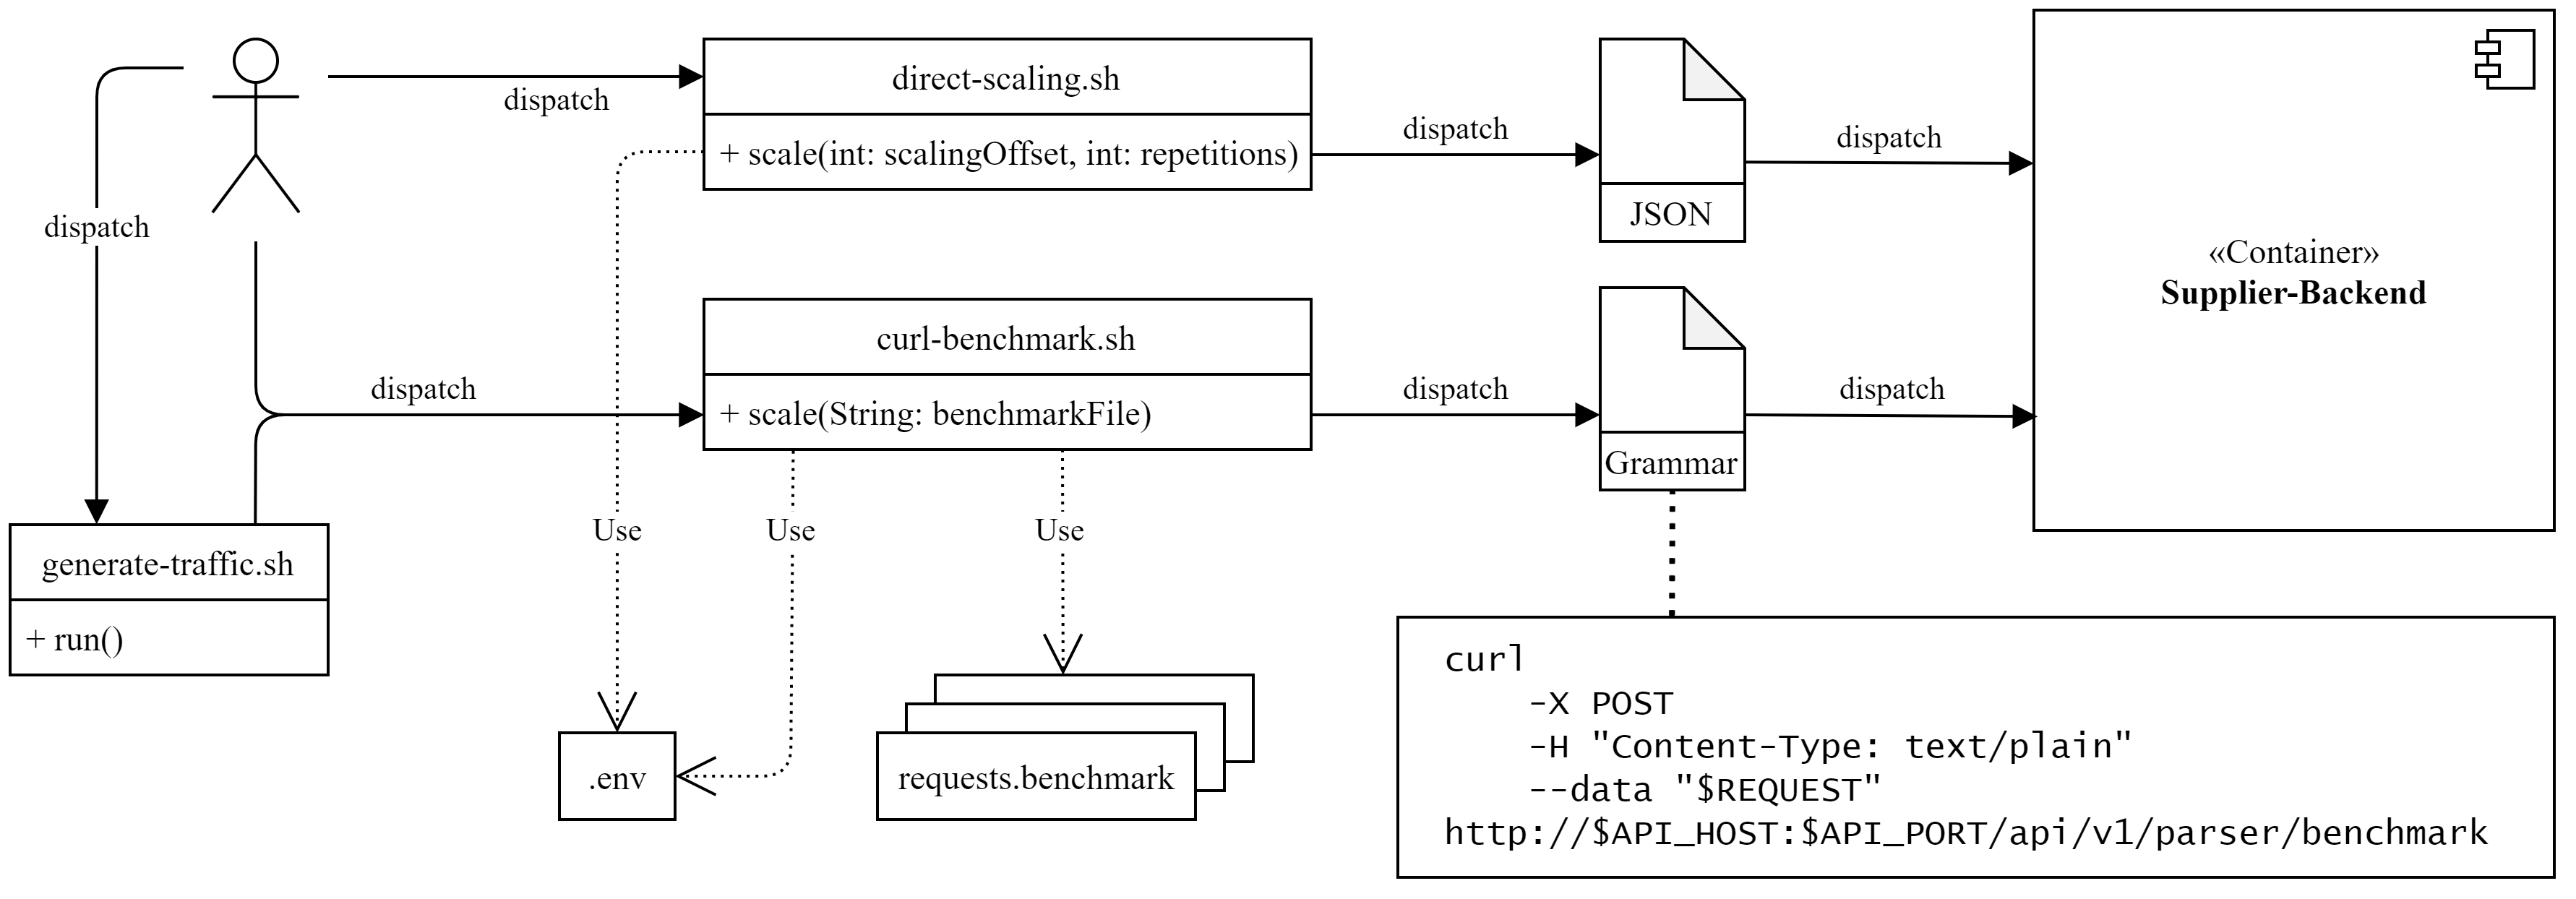
\includegraphics[width=\linewidth]{kapitel/problemloesung/implementierung/_img/input-uml}
	\caption[Bash Input UML]{Bash Input UML}
	\label{fig:bashOverview}
\end{figure}

\begin{itemize}
  \item \emph{direct-scaling}: bietet die Möglichkeit eine direkte Skalierungsanfrage an das System zu senden, ohne Payment-Messages verwenden zu müssen. Als Parameter werden die Skalierungsanzahl sowie die Wiederholungen erwartet (genauere Erklärung siehe \ref{erklaerungDirScal}).
  \item \emph{curl-benchmark}: sendet eine Skalierungsanfrage mit dem Dateiinhalt einer Datei, dessen Pfad als Eingabeparameter erwartet wird. Die Datei besitzt die Dateiendung \emph{.benchmark} wobei der Dateiinhalt einer spezifizierten Grammatik folgt (siehe \ref{lst:instruction-grammar}).
  \item \emph{generate-traffic}: dient vereinfachter Einstiegspunkt für den Benutzer. Hierbei werden rekursiv alle verfügbaren \emph{.benchmark} Dateien der Directory und übergibt diese der Reihe nach dem \emph{curl-benchmark} Skript.
\end{itemize}

Im folgenden Listing (siehe \ref{verb:scriptStruct}) ist ein Auszug der Projekt-Struktur abgebildet. Neben den genannten Skripts sind sämtliche \emph{.benchmark} Dateien nach services aufgeteilt in Unterordner aufgeteilt worden. Die \emph{.env} Datei beinhaltet die Verbindungsdaten zum Komponenten-Stack. Diese müssen bei der ersten Ausführung vom Benutzer angeglichen werden. Im Wesentlichen beschränkt sich das auf die IP-Adresse des Systems, falls der Benutzer in der Stack-Konfiguration entsprechende Änderungen vornimmt, sind diese hier ebenfalls zu vermerken.

\label{verb:scriptStruct}
\begin{minipage}{\linewidth}
\begin{lstlisting}[caption={Bash Skript - Struktur},style=bashStyle]
  $ tree request-scripts/ -a -L 3 --charset=ascii
  request-scripts/
  |-- curl-benchmark.sh
  |-- direct-scaling.sh
  |-- .env
  |-- generate-traffic.sh
  |-- README.md
  `-- requests
      |-- mixed
      |   |-- benchmark_large_mixed.benchmark
      |   |-- benchmark_medium_mixed.benchmark
      |   `-- benchmark_small_mixed.benchmark
      ...
\end{lstlisting}
\end{minipage}





% Damit eine direkte Skalierungsaufforderung an das System gesendet werden kann, wird folgender Endpunkt verwendet.

% \begin{verbatim}
%   curl "http://$HOST:$DIRECT_SCALING_PORT/manual-scale
%               ?additionalCnt=$CNT
%               &service=$SERVICE_NAME"
% \end{verbatim}

% Es handelt sich hierbei um eine Get-Anfrage an die \emph{Scaler-Proxy} Komponente des Stacks. Über die beiden Parameter "\emph{additionalCnt}" und "\emph{service}" lässt sich steuern wie viele neue Service Instanzen vom Orchestrator bereitgestellt werden sollen. Um dem Benutzer eine schlichtere Einstiegsmöglichkeit zu bieten, wurde das Skript \emph{direct-scaling.sh} implementiert (Inhalt siehe Listing \ref{lst:direct-scaling}). Dieses ist in der Lage automatisch eine Reihe von Anfragen an das System zu stellen. Vor der ersten Ausführung muss der Benutzer allerdings die IP-Adresse in der beiligenden .env Datei mit der seines Systems überschreiben.


\label{erklaerungDirScal}
\paragraph{Manuelles Skalieren}
Hierfür wird auf ein Bash-Skript namens "\emph{direct-scaling}" zurückgegriffen. Das Skript nimmt zwei Parameter entgegen. Der erste beschreibt die Anzahl der Instanzen, zu der das System skaliert werden soll, wobei hierbei eine inkrementelle Erhöhung von einer Instanz pro Durchlauf durchgeführt wird. Der Zweite Parameter gibt die Wiederholungen dieser testweisen Skalierung an. Der Aufruf \verb+./direct-scaling.sh 10 20+ resultiert beispielsweise darin, das sowohl für den Node.js als auch Spring Boot Service jeweils 10 Skalierungsschritte durchgeführt werden. Wenn zum Beispiel bereits ein Node.js Container läuft, wird im ersten Test eine weitere Instanz angefordert. Sobald die beiden Instanzen verfügbar sind, wird der Alert-Manager durch die Prometheus Komponente angewiesen die überflüssige Instanz zu löschen. Sobald wieder ein einziger Container verfügbar ist, wird dieser Schritt neunzehn weitere Male wiederholt. Nachdem dieser Schritt abgearbeitet wurde, erfolgt die nächste Skalierung bei der nun zwei neue Container kreiert werden sollen. Auch hier folgen 20 Wiederholungen. Diese Schritte werden solange durchgeführt bis zehn Container zwanzig Mal instanziiert wurden. 

\label{lst:direct-scaling}
\begin{minipage}{\linewidth}
\begin{lstlisting}[caption={direct-scaling},style=bashStyle]
...

request() {
  curl "http://$HOST:$DIRECT_SCALING_PORT/manual-scale?additionalCnt=$1&service=$4"
}

node_request() {request $1 $2 $3 'NODE'}
spring_request() {request $1 $2 $3 'SPRING'}

for scalingOffset in $(seq 1 $1)
do 
  for curr_rep in $(seq 1 $2)
	do 
    node_request $scalingOffset $curr_rep $2
    spring_request $scalingOffset $curr_rep $2
  done
done
\end{lstlisting}
\end{minipage}

\paragraph{Skalieren mithilfe von Grammatik}
Das beschriebene Skript sowie die der zugrunde liegende Http-Endpunkt bieten eine Möglichkeit, das Skalieren als Reaktion auf unbeantwortete Nachrichten zu umgehen. Um jedoch einen herkömmlichen Testdurchlauf zu starten greift der Benutzer auf einen Endpunkt vom \emph{Supplier} zurück: 

\begin{verbatim}
  curl 
    -X POST 
    -H "Content-Type: text/plain" 
    --data "$REQUEST" 
    "http://$API_HOST:$API_PORT/api/v1/parser/benchmark"
\end{verbatim}

Es handelt sich hierbei um eine POST-Anfrage. Im Body wird der Dateiinhalt eines für diesen Zweck verfassten Skripts angeheftet. Im Projekt wurden diverse Beispielskript verfasst. Diese liegen im Ordner \emph{./requests} und tragen die Dateiendung "\emph{.benchmark}". Der Inhalt korrespondiert zu einer spezifizierten Grammatik (siehe Listing \ref{lst:instruction-grammar}).

\label{lst:instruction-grammar}
\begin{verbatim}
  request     := batch*
  batch       := serviceName { instruction | instruction,* };
  serviceName := SPRING | NODE
  instruction := BENCHMARK ( messageCnt, duration ) | WAIT ( duration )
  messageCnt  := [0-9]+
  duration    := [0-9]+
\end{verbatim}

Es können beliebig viele Batchanfragen den Anfragenbody angeheftet werden. Eine Batch stellt in diesem Zusammenhang eine Gruppe an Skalierungsanfragen an einen bestimmten Service dar, wobei diese mindestens eine Skalierungsinstruktion enthalten muss. In diesem System gibt es zwei wesentliche Skalierungsinstruktionen: 

\begin{enumerate}
  \item BENCHMARK: Nimmt zwei Parameter entgegen. Der erste spezifiziert, wie viele neue Instanzen erstellt werden sollen, während der Zweite angibt, über welchen Zeitraum dies geschehen soll. Alle numerischen Angaben müssen einen positiven Zahlenwert enthalten. Da das System selbstständig in der Lage diese Instanzen wiederum auf ein gesetztes Minimum zu minimieren, wurde sich aktiv dagegen entschieden, das Herunterskalieren in die Grammatik aufzunehmen, um dem Benutzer eine möglichst schlicht gehaltene Schnittstelle zur Verfügung zu stellen.
  \item WAIT: Diese Instruktion erwartet lediglich einen Paramter, der angibt wie viele Millisekunden gewartet werden soll, bevor die nächste Instruktion dem System übergeben wird. 
\end{enumerate}


Damit der Benutzer allerdings direkt Anfragen ausführen kann, ohne sich mit der Grammatik beschäftigen zu müssen, wurde ein weiterer Skript-Aufsatz 
für das \emph{curl-benchmark} Skript entwickelt. Dieses trägt den Namen "\emph{generate-traffic.sh}" und sucht rekursiv absteigend in der eigenen Directory nach Dateien mit der entsprechenden Endung. Anschließend werden diese Skripte an das \emph{curl-benchmark} der Reihe nach als Parameter übergeben.


\todo{UI Erklärung einbinden...}



\subsubsection{Supplier Backend}
Bei dieser Komponente handelt es sich um ein Spring Projekt, dessen Aufgabe es ist, Benutzeranfragen in Nachrichten zu übersetzen, die vom System interpretiert und verarbeitet werden können. Die Schnittstelle für den Benutzer besteht hierbei aus einer REST-Api, die über Tools wie zum Beispiel curl angesprochen werden kann.


\paragraph{Implementierung}

\subparagraph{Generelle Spring Projektübersicht}
Da diese Komponente bezüglich der Struktur eines Spring-Projekts alle wesentlichen Merkmale besitzt, wird die genutzte Projektstruktur an dieser Stelle etwas näher erläutert. 

\label{verb:supplierStruct}
\begin{minipage}{\linewidth}
\begin{lstlisting}[caption={Supplier Backend - Struktur},style=bashStyle]
  $ tree stack/supplier-backend/ -a -L 7 --charset=ascii
  stack/supplier-backend/
  |-- Dockerfile
  |-- pom.xml
  `-- src
      `-- main
          |-- java
          |   `-- dps
          |       `-- hoffmann
          |           `-- producer
          |               |-- config
          |               |-- controller
          |               |-- model
          |               |-- properties
          |               |-- repository
          |               |-- response
          |               |-- service
          |               `-- SupplierBackendApplication.java
          `-- resources
              |-- application-dev.properties
              |-- application-prod.properties
              `-- application.properties
\end{lstlisting}
\end{minipage}

Das Muster, nach dem sämtliche Komponenten des Komponenten-Stacks entwickelt wurden, wird als \emph{Layered Architecture Pattern} oder \emph{n-tier pattern} bezeichnet \cite{oreilly-layered-arch}. Es stellt einen weitverbreiteten Standard in Java Enterprise Applikationen dar und zeichnet sich durch die klare Unterteilung der verschiedenen Hierarchien aus (siehe Abbildung \ref{fig:layeredArchitecture}). Sämtliche Packages innerhalb der Spring-Projekte finden sich innerhalb einer der Layer wieder. Es sei ebenfalls hervorzuheben, dass sämtliche Layer stets nur mit ihren direkt angrenzenden Schichten kommunizieren. Dies stellt ein weitaus übersichtlicheres Design sicher.

\begin{figure}[ht!]
	\centering
	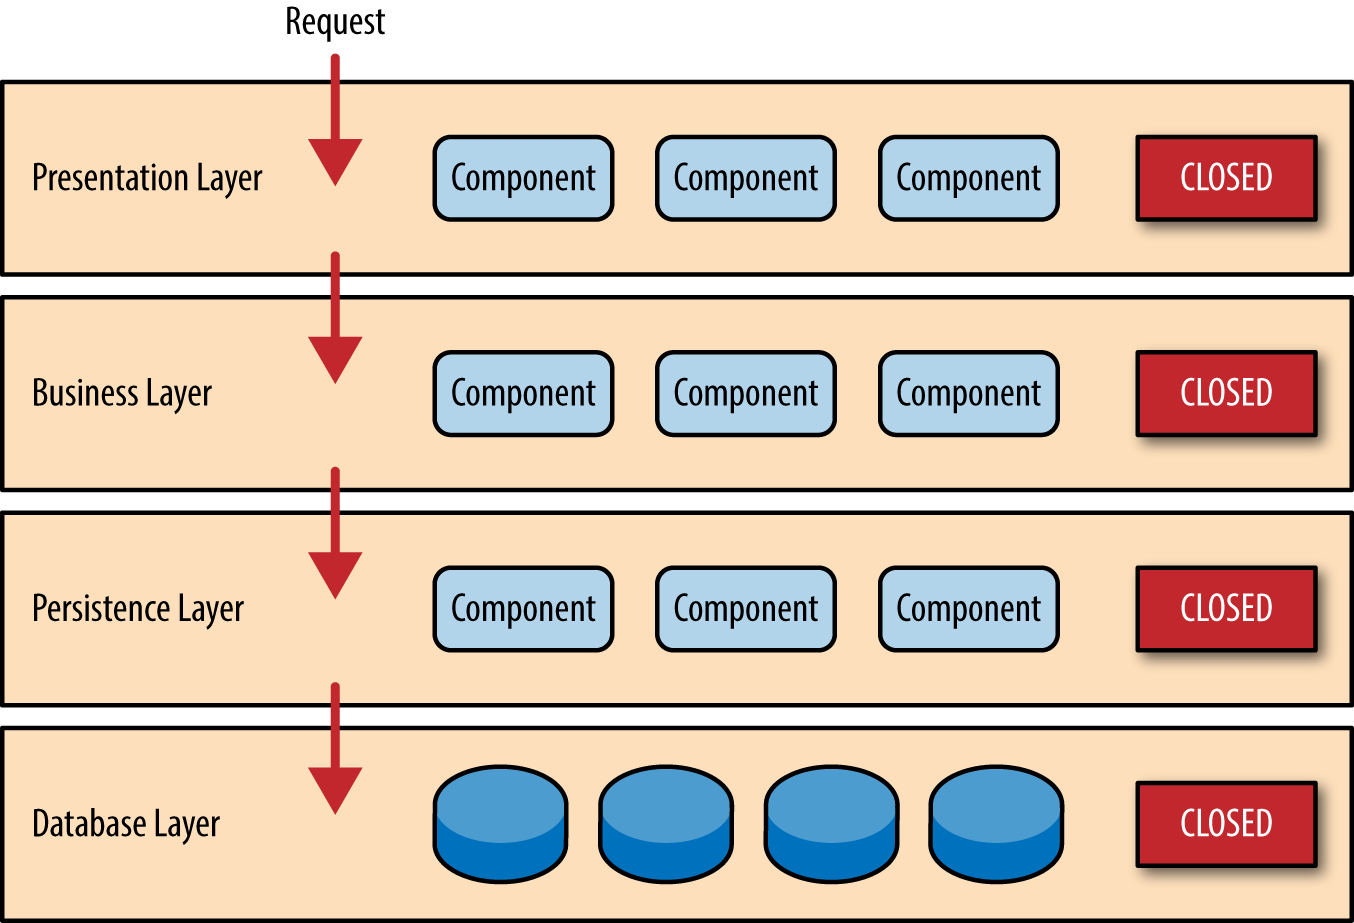
\includegraphics[width=.7\linewidth]{kapitel/problemloesung/implementierung/_img/dataflow-overview-01}
	\caption[Layered Architecture]{Layered Architecture \cite{oreilly-layered-arch}}
	\label{fig:layeredArchitecture}
\end{figure}


\begin{itemize}
  \item \emph{controller}: Dieses Package stellt alle Klassen bereit, welche direkt vom Benutzer angesprochen werden. Typischerweise handelt es sich zumindest im implementierten Stack um Rest-Schnittstellen, aber auch andere Typen (Soap, etc.) bieten entsprechende Implementierung. Klassen dieses Packages werden allgemeinhin als Controller bezeichnet und bilden eine erste Interaktionsschicht, welche keinerlei Business-Logik enthält. Bei diesem Package handelt es sich um einen Teil des Presentation Layers. Die Daten werden angenommen aber nicht direkt verarbeitet. Dies geschieht in sogenannten Services, welche spezifische Funktionalität implementieren. Controller dienen hierbei als ein Verteiler der eingehenden Nachrichten zu diesen Services. Die Service-Instanzen werden den Controllern Über den Spring-Context mittels Dependency Injection bereitgestellt, sodass sich der Entwickler selbst sich nicht mit der Instanziierung etc. zu beschäftigen braucht. 

  \item \emph{service}: Dieses Package enthält ausschließlich Service Implementierungen. Ein Service stellt einen logischen Funktionsbaustein der Anwendung dar und kann in den Spring-Context injected werden.

  \item \emph{repository}: Spring bietet über das Framework die JPA Implementierung \emph{Hibernate} nativen Support für die Anbindung an eine Datenbankverbindung. Dieses Package enthält Interfaces welche die Treiberschnittstelle beerben. Mit Hilfe spezifizierter Namenskonventionen ist es möglich Methodensignaturen Datenbankanfragen zu gestalten. Das Framework generiert hieraus die entsprechenden SQL-Abfragen.

  \item \emph{config}: Klassen dieses Packages konfiguieren instanziieren beziehungsweise konfigurieren Spring-Beans. Es gibt bei vielen voreingestellten Spring-Komponenten die Möglichkeit Beans über Annotations in der implementierenden Klasse zu erzeugen, in bestimmten Situation wird jedoch Zugriff auf die Instanz selbst zum Initialisierungszeitpunkt gebraucht um entsprechende Konfigurationsschritte zu unternehmen. Dies geschieht standardmäßig in diesem Package.

  \item \emph{model}: Klassen welche lediglich zum Abbilden bestimmter Datensätze genutzt werden, residieren in diesem Package. Hierbei ist es irrelevant ob es sich um JPA-Entitäten oder herkömmliche POJOs handelt.

  \item \emph{properties}: Spring bietet die Möglichkeit Daten aus den Konfigurationsdateien innerhalb der Resources direkt in den Application-Context zu laden.
  
  \item \emph{utils}: Klassen, die lediglich mit Business-Logik gefüllt sind und nicht vom Spring-Container verwaltet werden, sondern direkt im Programmcode instanziiert beziehungsweise aufgerufen werden, residieren in diesem Package.
  
  \item \emph{resources}: Die genutzte Verbindungs-Konfiguration zwischen Komponenten des Stacks werden innerhalb der \emph{.properties} Dateien verwaltet. Es ist möglich diese Information über den Dependency-Injection-Mechnismus innerhalb der Klassen hierauf zuzugreifen.

\end{itemize}


\subparagraph{Programmfluss}
Im folgenden UML-Diagramm (siehe Abbildung \ref{fig:supplierUml}) wurden ein Teil der Klassen des Suppliers dargestellt. Es wurde sich hierbei auf die wesentlichen Logikbausteine konzentriert. 

\begin{figure}[ht!]
	\centering
	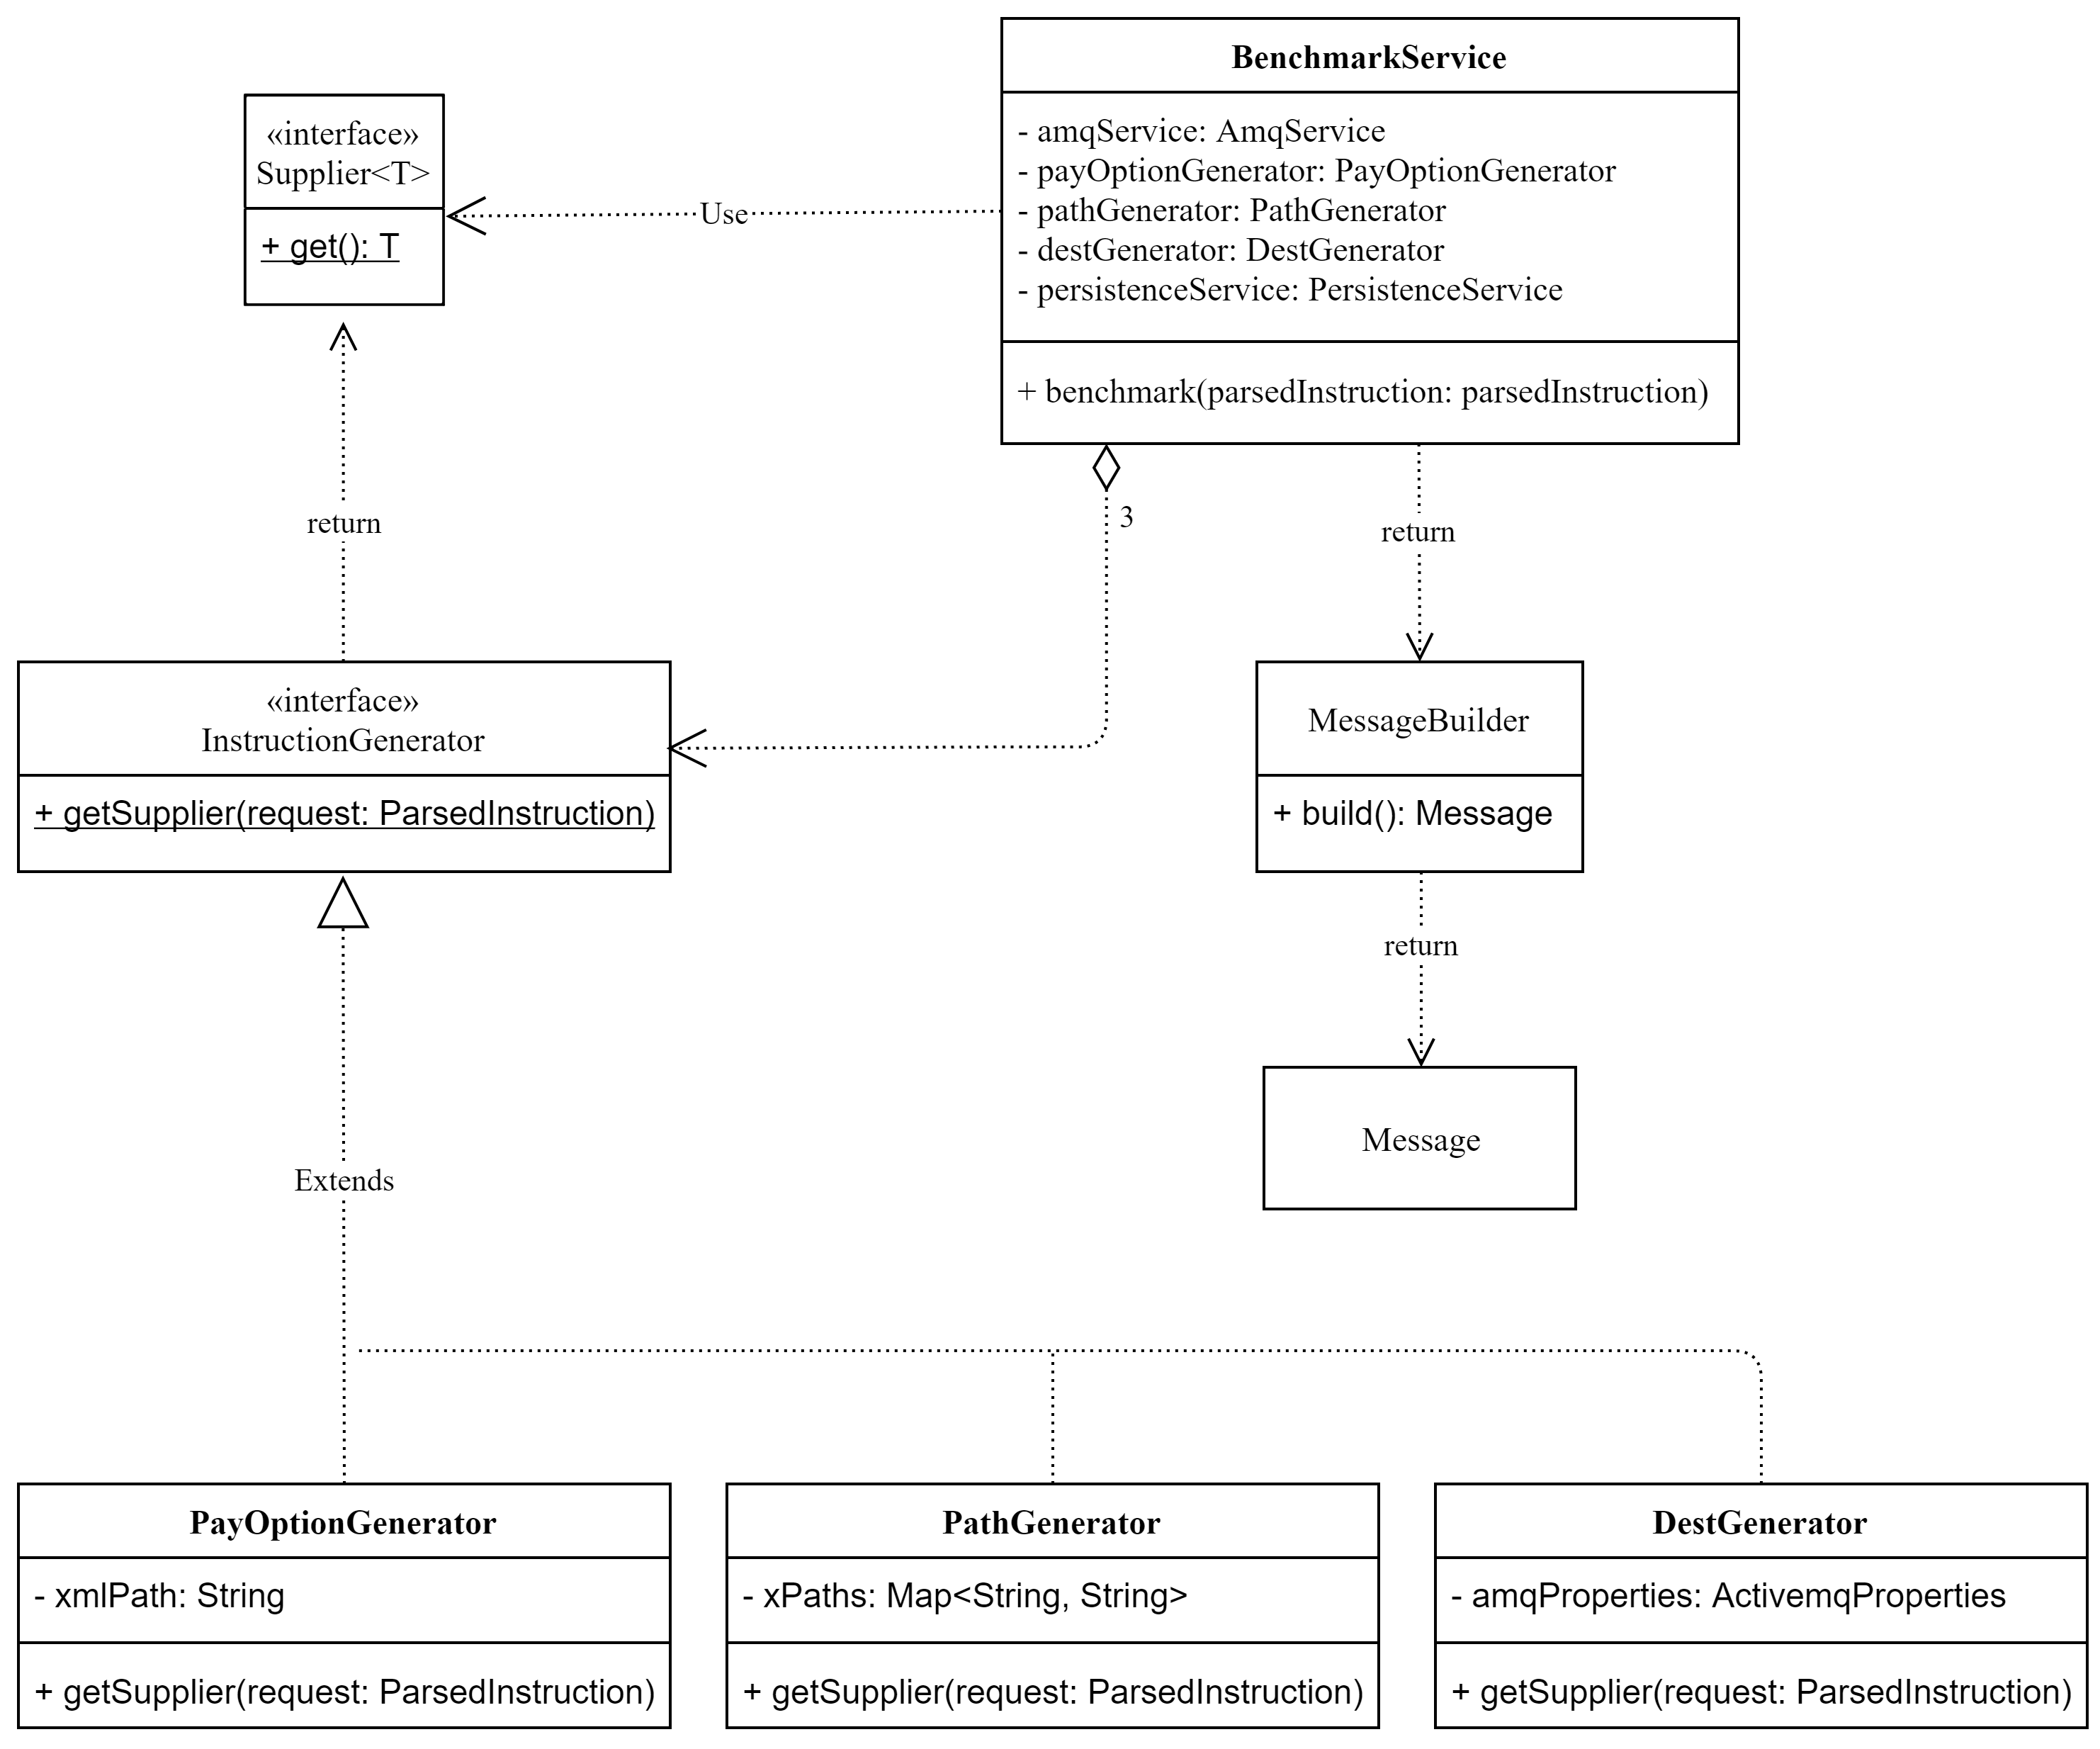
\includegraphics[width=\linewidth]{kapitel/problemloesung/implementierung/_img/supplier-uml}
	\caption[Backend Supplier UML]{Backend Supplier UML}
	\label{fig:supplierUml}
\end{figure}

Es gibt im primär zwei Einstiegspunkte für den Programmfluss. Der Benutzer möchte mithilfe der Benutzeroberfläche oder eines \emph{curl}-Aufrufs neue Nachrichten generieren, oder es wird auf die Dateiinhalte, die einer Grammatik folgen zurückgegriffen. Bei beiden Endpunkten wird im Controller eine Instanz vom Typ \emph{ParsedInstruction} erstellt. Diese enthält alle relevanten Informationen, die vom verarbeitenden \emph{BenchmarkService} gebraucht werden. Bei der Api-Anfrage durch den Curl-Aufruf lässt sich das Instanziieren direkt über das Parsen vom empfangenen Json umsetzen, während bei der Grammatik ein weiterer Service (\emph{RequestParserService}) verwendet wird, der aus der erhaltenen Grammatik diverse \emph{ParsedInstruction} Instanzen erstellt.

Wie im UML-Diagramm zu erkennen, werden aus der erhaltenen Instruktions-Instanz über verschiedene Generator-Implementierungen diverse Callbacks erstellt, die zum absetzen der Nachrichten in das System genutzt werden. Ein Auszug des zugrundeliegenden Codes folgt in Listing \ref{lst:supplierServiceImpl};

\begin{minipage}{\linewidth}
\begin{lstlisting}[style=javaStyle,caption={Supplier - Service},label=lst:supplierServiceImpl]
  
      ...

      // create generator instances
      Supplier<String> xPathSupplier = pathGenerator.getSupplier(parsedInstruction);
      Supplier<String> paymentSupplier = payOptionGenerator.getSupplier(parsedInstruction);
      Supplier<String> destinationSupplier = destGenerator.getSupplier(parsedInstruction);
      BiConsumer<PaymentMessage, Supplier<String>> amqConsumer =
              amqService.getConsumer(sessionIsTransacted);

      ...

      for (int i = 0; i < parsedInstruction.getMessageCnt(); i++) {

          // use generator instances to dynamically create message
          PaymentMessage payment = PaymentMessage.builder()
                  .batchId(batchId)
                  .xPath(xPathSupplier.get())
                  .content(paymentSupplier.get())
                  .sentTimestamp(now())
                  .build();

          amqConsumer.accept(payment, destinationSupplier);

          Thread.sleep(durationMillis);
      }
  }

  ...
  
\end{lstlisting}
\end{minipage}

In dem beschriebenen Listing ist zu erkennen, wie diese Generatoren genutzt werden. Sie extrahieren aus der gegebenen Instruktion-Instanz die jeweils relevanten Werte für ihren Anwendungsfall (Zeile 5 -- 9) und können bei der Erstellung der Nachrichten als Callback verwendet werden, und dynamisch neue Werte erstellen (Zeile 16 -- 21). Der Grund warum hierbei auf diese Callback-Struktur zurückgegriffen wurde, ist der, dass die gegebenen Werte in der Instruktion selbst als Instruktionen verstanden werden sollen. 

\subparagraph{Beispiel xPathSupplier} 
Der XPath gibt an, welches XML-Element bei der Verarbeitung durch den Konsumer im Detail extrahiert werden soll (bspw. IBAN, Betrag etc.). Es ist jedoch auch möglich, dass der Benutzer bei der API-Anfrage hierbei keinen genauen XPath angibt sondern möchte, dass hierbei ein beliebiges Element extrahiert werden soll. Dazu wird der Wert "\emph{Randomize}" in die Instruktion eingetragen. Dies ist sinnvoll um etwas Variation in die spätere Verarbeitung zu bekommen um bessere Messwerte erzielen zu könnnen. Im System wurden hierfür beispielhaft einige XPath Pfade manuell hinterlegt. Der Supplier hat intern Zugriff auf diese Sammlung. Je nachdem ob ein spezifischer Wert ausgegeben werden oder dieser variieren soll, wird stets der selbe Wert oder aber unterschiedliche Werte ausgegeben. Ähnliches gilt für die anderen verfügbaren Generator-Instanzen.


\subsubsection{Konsumer-Komponente}

Im folgenden UML-Diagramm ist die grundlegende Klassenstruktur der beteiligten Logikbausteine des Spring-Konsumenten zu erkennen. Da das Node.js Projekt einen sehr ähnlichen Aufbau besitzt, wird im folgenden lediglich der Ablauf der Spring Komponente zusammengefasst. Sämliche Informationen lassen sich jedoch nahtlos auf die Node.js Umgebung übertragen. 

\begin{figure}[ht!]
	\centering
	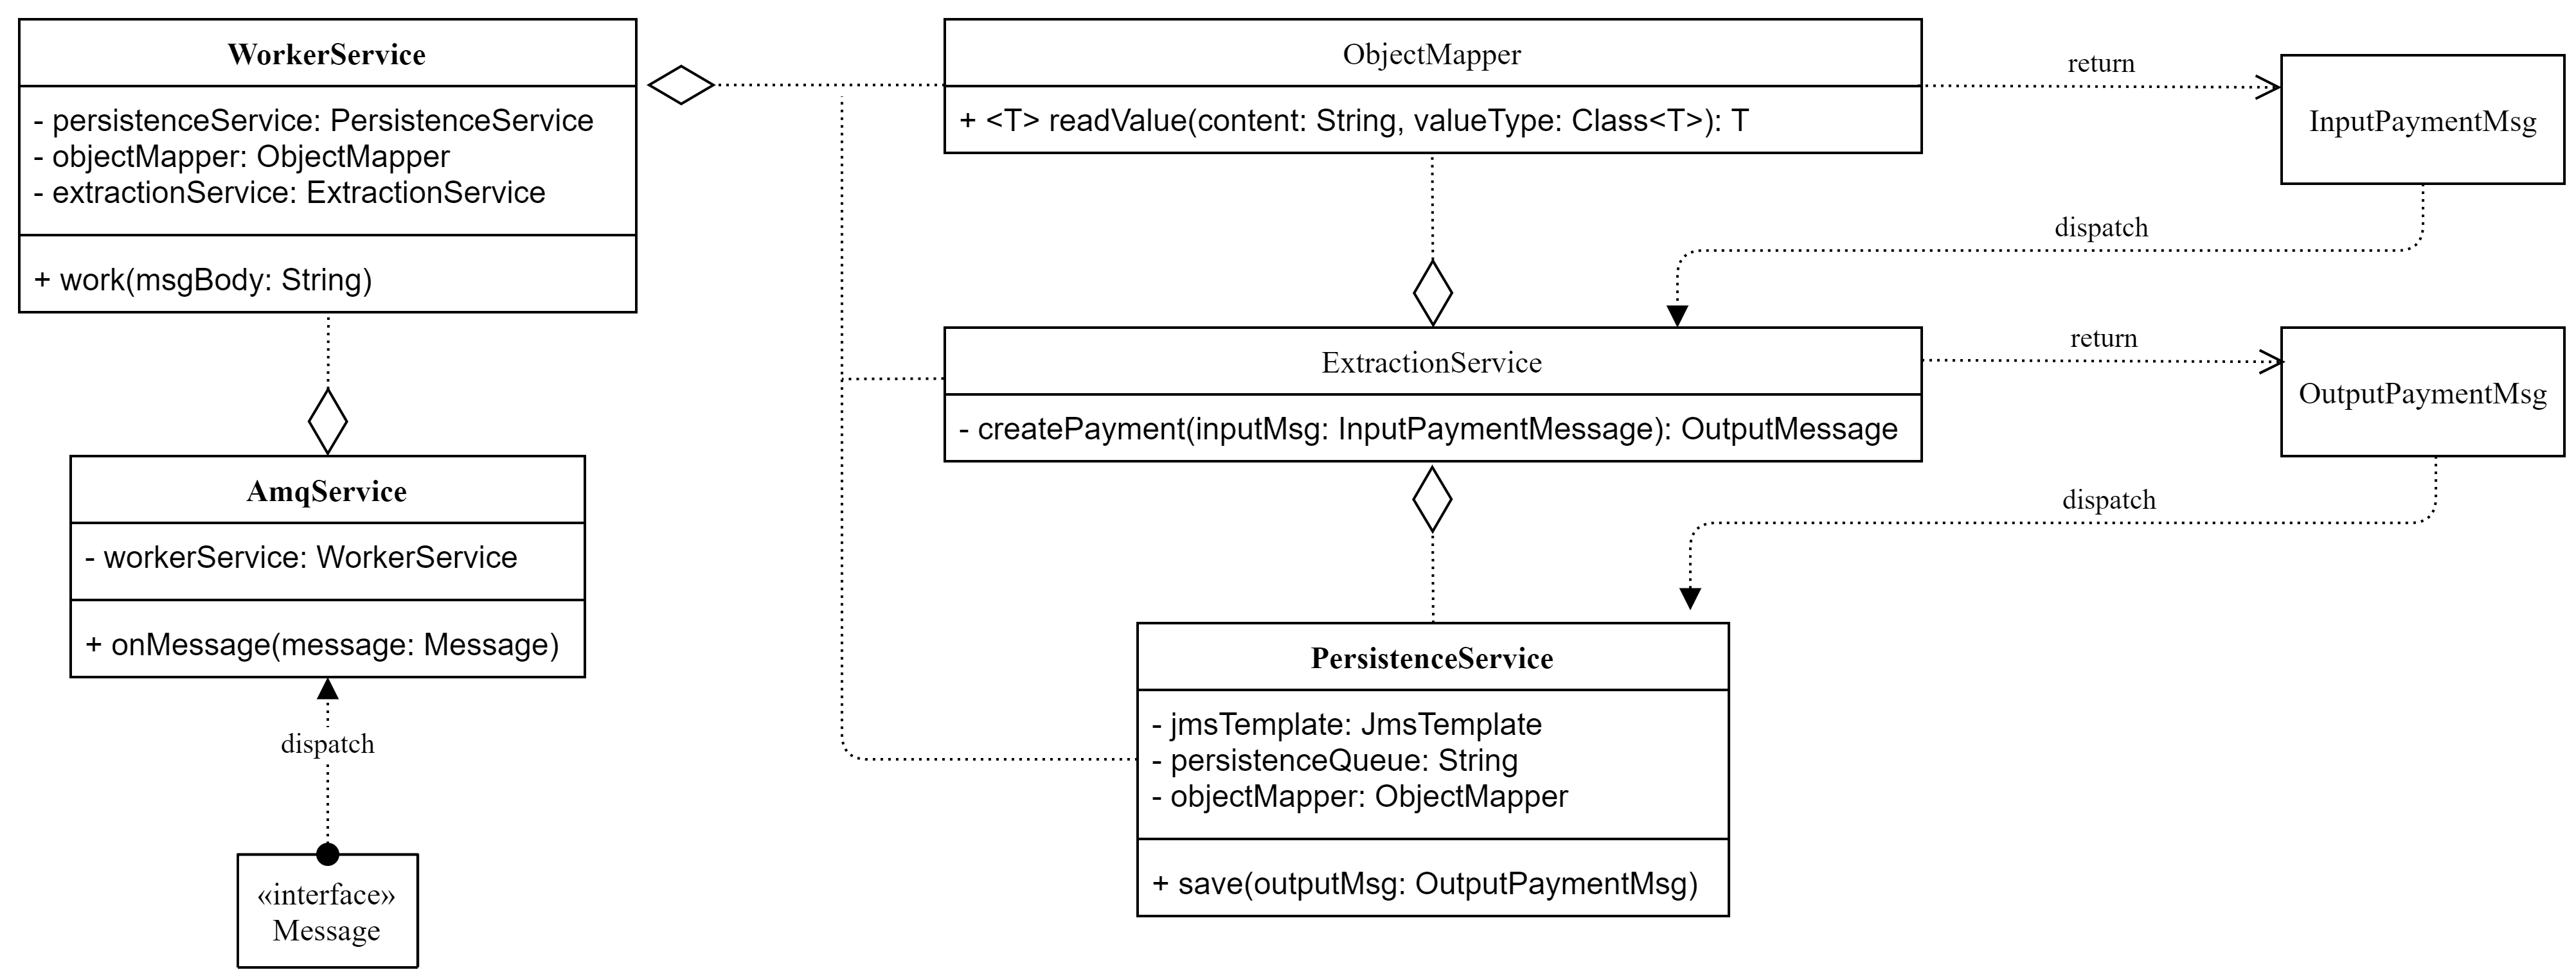
\includegraphics[width=\linewidth]{kapitel/problemloesung/implementierung/_img/consumer-uml}
	\caption[Consumer UML]{Consumer UML}
	\label{fig:consumerUml}
\end{figure}

Der Einstiegspunkt für den Spring-Konsumenten stellt der \emph{AmqService} dar. Nachrichten werden mithilfe dieser Komponente aus der Warteschlange des ActiveMq Brokers ausgelesen und an den \emph{WorkerService} delegiert. Über eine \emph{ObjectMapper} Instanz wird aus dem übergebenen String eine Objektinstanz eines Datenobjektes (\emph{InputPaymentMessage}) geniert (siehe Listing \ref{lst:consumerLogic}). Dieses Objekt wird an einen weiteren Service übergeben, der ein Element entsprechend der Vorgaben im Datenobjekt extrahiert. Wenn das zugrundeliegende XML nicht XSD konform ist oder das Element zum spezifizierten Pfad nicht gefunden werden kann, wird eine Null-Referenz ausgegeben. Es folgt ein Nullcheck bevor die Nachricht der Persistenzschicht übergeben wird.

\begin{minipage}{\linewidth}
\begin{lstlisting}[style=javaStyle,caption={WorkerService - Konsumer Logik},label=lst:consumerLogic]

  ...

  @SneakyThrows
  public void work(String msgBody) {
    InputPaymentMsg inputMessage = objectMapper.readValue(msgBody, InputPaymentMsg.class);
    OutputPaymentMsg outputMessage = extractionService.createPayment(inputMessage);
    if (outputMessage != null) {
      persistenceService.save(outputMessage);
    }
    Thread.sleep(3000);
  }

  ...

\end{lstlisting}
\end{minipage}


\subsubsection{Scaler Proxy}

Im folgenden UML-Diagramm (siehe Abbildung \ref{fig:proxyScalerUml}) wird die grundlegende Klassenstruktur der Scaler-Proxy-Komponente zusammengefasst. 

\begin{figure}[ht!]
	\centering
	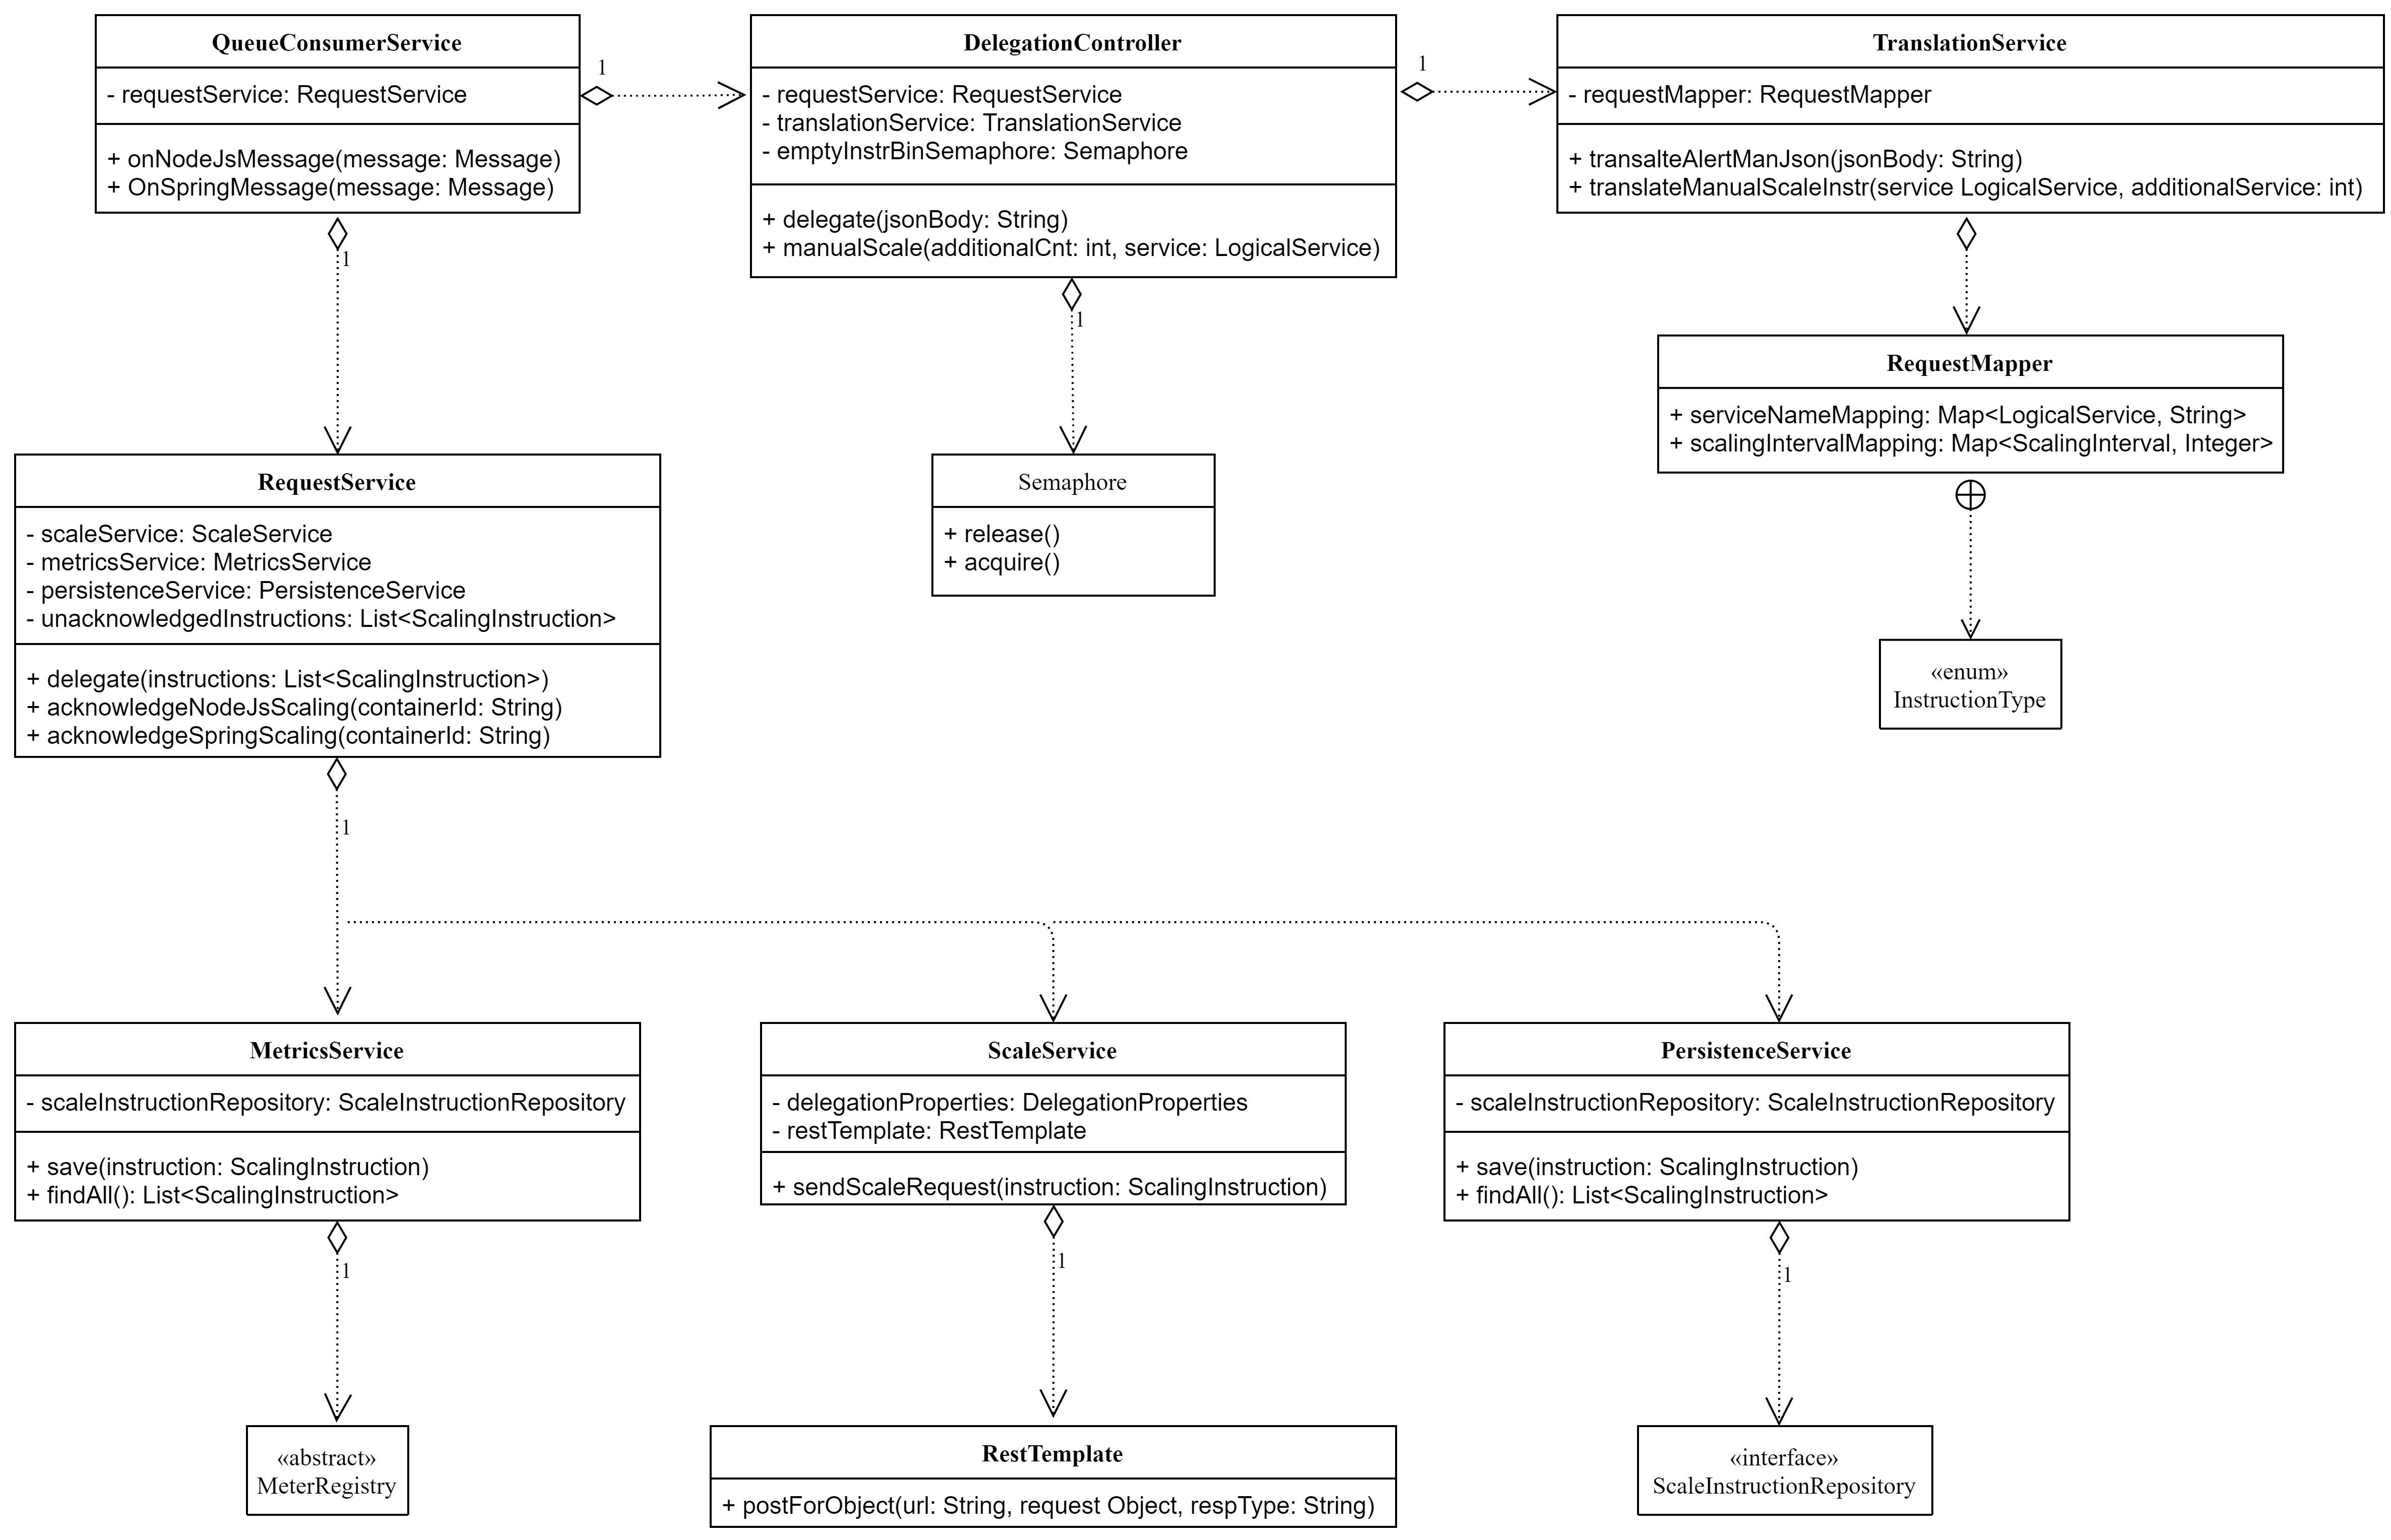
\includegraphics[width=\linewidth]{kapitel/problemloesung/implementierung/_img/scaler-proxy-uml}
	\caption[Scaler-Proxy UML]{Scaler-Proxy UML}
	\label{fig:proxyScalerUml}
\end{figure}


% In Listing \ref{lst:supplierBenchmarkEndpoint} ist die Definition desjenigen Endpunktes zu erkennen, der als primärer Einstiegspunkt für die eingehenden Anfragen der Benutzeroberfläche gilt. Sobald der Benutzer eine Eingabe tätigt und der Endpunkt angesprochen wird, übersetzt eine Objectmapper Instanz den erhaltenen String in eine Datenstruktur, welche alle relevanten Informationen enthält. Die Methode wurde außerdem mit einer \emph{Transactional}-Annotation versehen, die es ermöglicht das Übermitteln mehrere Nachrichten an eine Queue in einer Transaktion durchzuführen (siehe \todo{Referenz} einfügen), dies wird im späteren Verlauf von Bedeutung sein. Im Spring-Framework muss jedoch bereits der Einstiegspunkt mit einer solchen Annotation versehen werden, um zu gewährleisten, dass die aufgerufenen Logikbausteine alle im selben Transaktion-Kontext ausgeführt werden \todo{Quelle?}.



% \begin{lstlisting}[style=javaStyle,caption={Supplier - Endpunkt},label=lst:supplierBenchmarkEndpoint]

%   ...

%   @Transactional(propagation = Propagation.REQUIRES_NEW)
%   @RequestMapping(value = "/start",
%           method = POST,
%           consumes = APPLICATION_JSON_VALUE)
%   public void startPaymentBenchmark(@RequestBody String jsonBody) throws JsonProcessingException {
%       log.info("new benchmark request: {}", jsonBody);
%       ParsedInstruction req = mapper.readValue(jsonBody, ParsedInstruction.class);
%       benchmarkService.benchmark(req);
%   }

%   ...
  
% \end{lstlisting}




% \begin{lstlisting}[style=javaStyle,caption={Supplier - Service},label=lst:supplierServiceImpl]

%   ...

%   @SneakyThrows
%   @Transactional
%   public void benchmark(ParsedInstruction parsedInstruction) {
%       parsedInstruction.setReceived(now());
%       // set batch id by saving it to db and reloading instance
%       parsedInstruction = persistenceService.save(parsedInstruction);
%       int batchId = parsedInstruction.getMessageId();
%       boolean sessionIsTransacted = sessionIsTransacted(parsedInstruction);

%       Supplier<String> xPathSupplier = pathGenerator.getSupplier(parsedInstruction);
%       Supplier<String> paymentSupplier = payOptionGenerator.getSupplier(parsedInstruction);
%       Supplier<String> destinationSupplier = destGenerator.getSupplier(parsedInstruction);
%       BiConsumer<PaymentMessage, Supplier<String>> amqConsumer =
%               amqService.getConsumer(sessionIsTransacted);

%       int durationMillis = 0;
%       if (!sessionIsTransacted) {
%           durationMillis = parsedInstruction.getDuration()
%                   / (parsedInstruction.getMessageCnt() - 1);
%       }

%       for (int i = 0; i < parsedInstruction.getMessageCnt(); i++) {

%           PaymentMessage payment = PaymentMessage.builder()
%                   .batchId(batchId)
%                   .xPath(xPathSupplier.get())
%                   .content(paymentSupplier.get())
%                   .sentTimestamp(now())
%                   .build();

%           amqConsumer.accept(payment, destinationSupplier);

%           Thread.sleep(durationMillis);
%       }
%   }

%   ...
  
% \end{lstlisting}

% In Listing \ref{lst:supplierServiceImpl} ist zu erkennen, wie die Abarbeitung einer übersetzten Nachricht im Detail erfolgt.

% \begin{itemize}
%   \item Zeile 7: Zu Beginn wird der aktuelle Timestamp an die übersetzte Nachricht angeheftet, um im Nachhinein diverse Messwerte berechnen zu können.

%   \item Zeile 9: Die übersetzte Nachricht wird in der Datenbank hinterlegt.

%   \item Zeile 11: Da die gesamte Methode mit einer weiteren \emph{Transactional-Annotation} versehen wurde, ist es möglich beim Absenden der Nachrichten einen transaktionbasierten Ansatz zu wählen. Es muss jedoch bereits an dieser Stelle entschieden werden, ob dies tatsächlich nötig ist. Hierfür wird das übersetzte Datenobjekt entsprechend untersucht. 

%   \item Zeile 13: Abhängig von der gegebenen Instruktion ist es möglich unterschiedliche Felder eines Payments auszulesen. Es gibt beispielsweise die Möglichkeit eine IBAN, den Betrag der Überweisung, den Empfänger etc. zu extrahieren. An dieser Stelle wird ein entsprechender Supplier erzeugt, der im späteren Verlauf diese Information liefert und das standardisierte Java Interface des Function-Modules implementiert. Der Grund diese Funktionalität in eine Callback Funktion ausgelagert wurde, ist der, dass es möglich sein soll, dass sich die Ausgabe über Zeit ändern kann. So kann der Benutzer beispielsweise in der Nachricht angeben, dass er zufällige Datenfelder pro Nachricht ausgeben möchte. Bei Nachricht X, soll zum Beispiel das IBAN-Feld und bei Nachricht Y der Betragswert bestimmt werden. Diese Maßnahme wurde lediglich ergriffen um etwas Variation der Messwerte hinsichtlich der Verarbeitungsdauer zu generieren.

%   \item Zeile 14: Selbes gilt für die Nachricht selbst. Es soll möglich sein, dem Benutzer die Wahl zu lassen, ob dieser die Benchmark-Tests stets mit der gleichen beispielhaften Payment-Nachricht durchführen möchte oder nicht. Falls ja soll Nachrichten mit zufälligen Werten zum Beispiel für die IBAN etc. zu generiert werden. In diesem Protoypen wurde allerdings lediglich das Design für die Funktionalität entwickelt, da es im Endeffekt keinen Einfluss auf die generierten Metriken hat welche Daten im Detail in dem XML-Inhalt hinterlegt wurden.

%   \item Zeile 15: Diese Callback Funktion gibt den Warteschlangennamen aus zu dem die generierten Nachrichten geschickt werden sollen.
  
%   \item Zeile 16: Abhängig davon, ob es sich um eine Anfrage, die in einer Transaktion durchgeführt werden soll oder nicht, wird für das Callback eine Spring-Bean zur Datenübermittlung zum Message-Broker verwendet, die mit einem Transaction Flag versehen wurde oder nicht. In Listing \ref{lst:supplierBiConsumer} ist erkenntlich, dass hierbei je nach gesetztem Flag eine Auswahl eines vorkonfigurierten JmsTemplates erfolgt. Dieses Template stellt eine weitere Abstraktionsstufe zwischen Komponente und Broker dar. Sie wird vom Framework gestellt, die Verbindung muss jedoch über Klassen im \emph{config} Package konfiguriert werden. Diese Funktion stellt beim Absenden der Nachrichten die Schnittstelle zum Messagebroker dar.

%   \item Zeile 27: Es werden Nachrichten generiert, die von den weiteren Stack-Komponenten verarbeitet werden können.

%   \item Zeile 34: Die Nachrichten werden an die Broker-Schnittstelle übergeben.

%   \item Zeile 36: Je nachdem ob bei der eingegangenen Nachricht ein Zeitraum angegeben wurde über den die Nachrichten abgeschickt werden soll, wird an dieser Stelle ein entsprechender Sleep-Aufruf durchgeführt.

% \end{itemize}


% \begin{lstlisting}[style=javaStyle,caption={Supplier - Bi Consumer},label=lst:supplierBiConsumer]

%   ...

%   public BiConsumer<PaymentMessage, Supplier<String>> getConsumer(boolean sessionIsTransacted) {
%     return sessionIsTransacted
%             ? (message, destGen) -> sendObjPaymentQueueMessage(
%               transactedJmsTemplate, message, destGen)
%             : (message, destGen) -> sendObjPaymentQueueMessage(
%               nonTransactedJmsTemplate, message, destGen);
%   }

%   ...

% \end{lstlisting}


% \subparagraph{Programmfluss - Endpunkt Eingabedatei}
% Da die Lastentests primär mit Hilfe diverser Bash-Skripte ausgeführt werden, gibt es einen weiteren Endpunkt für diesen Anwendungsfall. Nachdem Textnachrichten auf die Grammatik geprüft und in eine Objektstruktur konvertiert wurden, über die iteriert werden kann, wird allerdings die selbe Schnittstelle wie schon beim Gui-Aufruf angesteuert, da sich die darunter liegende Logik in keinster Weise unterscheidet. In Listing \ref{lst:supplierParserEndpoint} ist der erwähnte Endpunkt zu erkennen.

% \begin{lstlisting}[style=javaStyle,caption={Supplier - Bi Consumer},label=lst:supplierParserEndpoint]
%   @Autowired
%   private RequestParserService parserService;

%   @Transactional(propagation = Propagation.REQUIRES_NEW)
%   @RequestMapping(value = "/benchmark",
%           method = POST,
%           consumes = TEXT_PLAIN_VALUE)
%   public void parseBenchmark(@RequestBody String textValue) {
%       new Thread(() -> parserService.runRequest(textValue)).start();
%   }
% \end{lstlisting}

% Ähnlich wie bei ersten Endpunkt gibt es wieder ein Transaktion-Context eröffnet. Bezüglich der Http-Anfrage hat sich lediglich geändert, dass nun anstatt eines Json-Wertes eine Textnachricht erwartet wird, da die hinterlegte Grammatik nicht mit einem Json-Format kompatibel ist \todo{schauen ob Grammatik ueberhaupt vorher erklaert wurde}. Um zu ermöglich, dass mehrere Benchmark Dateiinhalte das System direkt hintereinander mit Werten versorgen kann, wird hier mit jeder eingehenden Anfrage ein neuer Thread gestartet. Dies stellt auch sicher, dass die Anfragen direkt hinterlegt werden und alte Anfragen nicht erst abgearbeitet werden müssen bevor neue angenommen werden können. Der Zwischenschritt des Übersetzens der Grammatik in tatsächlich ausführbare Anweisung erfolgt in einer dedizierten Service-Komponente. Damit es zu keiner Verfälschung der Ergebnisse kommt, ist es von größter Bedeutung, dass lediglich nur ein einziger Thread mit der Ausführung der eigentlichen Tests zur Zeit betraut wird. Wenn es hierbei zu einem nebenläufigen Verhalten kommen sollte, würde dies die verfügbaren Resourcen einschränken und die Werte würden Ungenauigkeiten aufweisen, was es unter allen Umständen zu vermeiden gilt. Um diesem Problem entgegenzuwirken, wurde im \emph{Parser-Service} eine Semaphore eingeführt, die sicherstellt, dass stets nur ein Thread arbeitet. Das Ausführen einer Anfrage wird demnach in einem kritischen Abschnitt ausgeführt. \todo{weiterschreiben}








\subsubsection{Spring Boot}

% $ tree spring-consumer/ -L 7
% spring-consumer/
% ├── Dockerfile
% ├── pom.xml
% └── src
%     └─ main
%        ├── java
%        │   └── dps
%        │       └── hoffmann
%        │           └── springconsumer
%        │               ├── config
%        │               ├── Main.java
%        │               ├── model
%        │               ├── service
%        │               ├── SpringConsumerApplication.java
%        │               └── utils
%        └── resources
%            ├── application-dev.properties
%            ├── application-prod.properties
%            ├── application.properties
%            └── docs
%                └── paymentSchema.xsd


\subsection{Node.js}

% \begin{lstlisting}[language=bash]
%  tree . -L 1
% .
% ├── Dockerfile
% ├── package.json
% ├── package-lock.json
% ├── specification.xsd
% ├── src
% └── tsconfig.json
% \end{lstlisting}
\todo{uncomment}

\subsubsection{Projektübersicht}
Das Projekt beinhaltet neben sämtlichen Quellcode-Dateien ein Dockerfile, eine package.json und eine tsconfig Konfigurationsdatei. 

\subparagraph{Dockerfile}
Bei dem verwendeten Dockerfile handelt es sich um eine multi-stage Konfiguration. \todo{Quellen raussuchen}

\todo{Zeilennummern}
\begin{lstlisting}[language=bash]
  # stage 1 building the code
  FROM node:10.15.3 AS builder
  WORKDIR /usr/app
  COPY package*.json ./
  RUN npm install
  COPY . .
  RUN npm run build 
  
  # stage 2
  FROM node:10.15.3-alpine
  WORKDIR /usr/app
  COPY package*.json ./
  RUN npm install --production
  
  COPY --from=builder /usr/app/dist ./dist
  
  COPY --from=builder /usr/app/schema.sql .
  COPY --from=builder /usr/app/specification.xsd .
  
  CMD node dist/src/index.js
\end{lstlisting}

\subparagraph{Typescript Konfiguration}

\subparagraph{Quellcode}


\begin{minipage}{\linewidth}
\begin{lstlisting}[style=bashStyle,caption={Node.js Projektstruktur},label=lst:nodeProjStruc]
  $ tree stack/node-consumer/ -a -L 3 --charset=ascii
  stack/node-consumer/
  |-- Dockerfile
  |-- .dockerignore
  |-- package.json
  |-- package-lock.json
  |-- schema.sql
  |-- scripts
  |   `-- buildimage.sh
  |-- specification.xsd
  |-- src
  |   |-- index.ts
  |   |-- model
  |   |   |-- PaymentInput.ts
  |   |   |-- PaymentMessage.ts
  |   |   `-- ResultWrapper.ts
  |   |-- service
  |   |   |-- AmqService.ts
  |   |   `-- WorkerService.ts
  |   `-- utils
  |       |-- ElementExtractor.ts
  |       |-- IdGenerator.ts
  |       `-- XsdChecker.ts
  `-- tsconfig.json
\end{lstlisting}
\end{minipage}


Die Programmlogik wurde in drei wesentliche packages aufgeteilt (siehe Listing \todo{Listing einkommentieren und referenzieren}). 

\begin{itemize}
  \item \emph{model}: Dieses Package beinhaltet sämtliche Datenstrukturen, die vom System zur Bearbeitung der eingehenden Nachrichten verwendet werden.
  \item \emph{model}: Dieses Package beinhaltet sämtliche Komponenten welche logisch klar abgetrennte Aufgabe implementieren und über Schnittstellen miteinander kommunizieren. Hierbei wurde sich an der Architektur einer typischen Spring-Anwendung orientiert.
  \item \emph{model}: Dieses Package beinhaltet sämtliche Funktionalität der abzuarbeitenden Businesslogik.
\end{itemize}





\section{Implementierung mittels Containerplattform}


\subsection{Build}
Um das Projekt im Komponenten-Stack als Dockercontainer zu deployen, muss in einem ersten Schritt ein Docker Image erstellt werden. Dieses kann im Anschluss als Container instanziiert werden. Zum Erstellen eines Docker-Images wird auf ein sogenannten "\emph{Dockerfile}" zurückgegriffen, das die Beschreibung des Build-Prozesses für dieses Image enthält. Da alle Spring-Projekte im Komponenten-Stack mit einem fast identischen Dockerfile versehen wurden, gilt die folgende Beschreibung in gleichem Maß für alle weiteren Spring-Projekte. \todo{Multistage Build erklären / Quelle raussuchen}

\begin{minipage}{\linewidth}
\begin{lstlisting}[style=javaStyle,caption={Supplier - Bi Consumer},label=lst:supplierParserEndpoint]
  FROM maven:3.8.1-openjdk-11 AS build
  COPY src /usr/src/app/src
  COPY pom.xml /usr/src/app
  RUN mvn -f /usr/src/app/pom.xml clean package -DskipTests

  FROM gcr.io/distroless/java
  COPY --from=build /usr/src/app/target/supplier-backend.jar /usr/app/supplier-backend.jar
  EXPOSE 9245
  ENTRYPOINT ["java","-jar","/usr/app/supplier-backend.jar"]
\end{lstlisting}
\end{minipage}

\begin{itemize}
  \item Zeile 1: Ein Dockerfile beginnt meist mit der Angabe eines sogenannten "\emph{Baseimages}". Dies kann eine minimale Linux Distribution sein, oder wie in diesem Fall ein System auf dem bereits diverse Konfigurationen definiert wurden. Bei dem verwendeten Image, wurde eine Java Runtime sowie das Buildprogramm \emph{maven} bereits vorinstalliert. Beides wird für die Ausführung des Spring-Projekts gebraucht. 
\end{itemize}







\subsection{Container Lifecycle}
\begin{itemize}
  \item Auf verschiedene Schichten eingehen
  \item Auf Ergebnisse beziehen
\end{itemize}
\subsection{Docker Swarm}

\begin{itemize}
  \item Prototypen im Detail erlaeutern
\end{itemize}


\renewcommand\theadalign{bc}
\renewcommand\theadfont{\bfseries}
\renewcommand\theadgape{\Gape[4pt]}
\renewcommand\cellgape{\Gape[4pt]}


\begin{minipage}{\linewidth}
\begin{lstlisting}[style=bashStyle,caption={Node.js Projektstruktur},label=lst:nodeProjStruc]
cat .env

# qbn: queue bound (level) n
# cbn: container bound (level) n

QB0=15
QB1=30
QB2=100
CB0=1
CB1=5
CB2=10
CB3=30
\end{lstlisting}
\end{minipage}


\begin{tabularx}
  {\textwidth}
  { X | X | X | X | X }
  \toprule
      \centering \hspace{4mm} \uline{QL3} \newline \footnotesize \textit{QB2 \textless{} MC} 
    & \centering \hspace{4mm} UP \newline \footnotesize \textit{abs(CB0 -- CB3)} 
    & \centering \hspace{4mm} UP \newline \footnotesize \textit{abs(CB1 -- CB3)} 
    & \centering \hspace{4mm} UP \newline \footnotesize \textit{abs(CB2 -- CB3)} 
    & \centering \hspace{4mm} OK \newline -- 
    \tabularnewline
  \hline
      \centering \hspace{4mm} \uline{QL2} \newline \footnotesize \textit{QB1 \textless{} MC $\leq$ QB2} 
    & \centering \hspace{4mm} UP \newline \footnotesize \textit{abs(CB0 -- CB2)} 
    & \centering \hspace{4mm} UP \newline \footnotesize \textit{abs(CB1 -- CB2)} 
    & \centering \hspace{4mm} OK \newline -- 
    & \centering \hspace{4mm} DOWN \newline \footnotesize \textit{abs(CB2 -- CB3)} 
    \tabularnewline
  \hline
      \centering \hspace{4mm} \uline{QL1} \newline \footnotesize \textit{QB0 \textless{} MC $\leq$ QB1} 
    & \centering \hspace{4mm} UP \newline \footnotesize \textit{abs(CB0 -- CB1)} 
    & \centering \hspace{4mm} OK \newline -- 
    & \centering \hspace{4mm} DOWN \newline \footnotesize \textit{abs(CB1 -- CB2)} 
    & \centering \hspace{4mm} DOWN \newline \footnotesize \textit{abs(CB1 -- CB3)} 
    \tabularnewline
  \hline
      \centering \hspace{4mm} \uline{QL1} \newline \footnotesize \textit{QB0 \textless{} MC $\leq$ QB1} 
    & \centering \hspace{4mm} UP \newline \footnotesize \textit{abs(CB0 -- CB1)} 
    & \centering \hspace{4mm} OK \newline -- 
    & \centering \hspace{4mm} DOWN \newline \footnotesize \textit{abs(CB1 -- CB2)} 
    & \centering \hspace{4mm} DOWN \newline \footnotesize \textit{abs(CB1 -- CB3)} 
    \tabularnewline
  \hline
      \centering \hspace{4mm} \uline{QL0} \newline \footnotesize \textit{QB0 == MC} 
    & \centering \hspace{4mm} OK \newline -- 
    & \centering \hspace{4mm} DOWN \newline \footnotesize \textit{abs(CB0 -- CB1)} 
    & \centering \hspace{4mm} DOWN \newline \footnotesize \textit{abs(CB0 -- CB2)} 
    & \centering \hspace{4mm} DOWN \newline \footnotesize \textit{abs(CB0 -- CB3)} 
    \tabularnewline
  \hline
    & \centering \hspace{4mm} \uline{CL0} \newline \footnotesize \textit{CB0 == MC} 
    & \centering \hspace{4mm} \uline{CL1} \newline \footnotesize \textit{CB0 \textless{} MC $\leq$ CB1} 
    & \centering \hspace{4mm} \uline{CL1} \newline \footnotesize \textit{CB1 \textless{} MC $\leq$ CB2} 
    & \centering \hspace{4mm} \uline{CL1} \newline \footnotesize \textit{CB2 \textless{} MC $\leq$ CB3} \tabularnewline
  \bottomrule
\end{tabularx}

\section{Implementierung Lasttest}
\subsection{Timeline}
\subsection{Testbedingungen}
\begin{itemize}
  \item Kommt in den Anhang
  \item hat Prof. zwar als eigenes Kapitel erwaehnt, bin mir aber nicht sicher ob das wirklich noetig ist
  \item auf welcher Hardware werden Tests durchgefuehrt?
  \item chaos monkey / Stoerfaelle erlaeutern
\end{itemize}

\begin{table}
  \centering
  \caption{Server Specs}
  \bigskip
  \begin{tabular}{ c l }
    \toprule
    Prozessor & Intel(R) Xeon(R) Gold 6226R CPU @ 2.90GHz \\
    \midrule
    Kerne & 6 Prozessoren á 16 Kerne \\
    \midrule
    RAM & 16 GB \\
    \midrule
    Storage & 150 GB \\
    \bottomrule
  \end{tabular}
\end{table}


\section{Implementierung Visualierung und Monitoring zur Unterst\"utzung der Auswertung}

% \begin{lstlisting}[language=bash]
%  tree . -L 1
% .
% ├── Dockerfile
% ├── package.json
% ├── package-lock.json
% ├── specification.xsd
% ├── src
% └── tsconfig.json
% \end{lstlisting}





\begin{itemize}
  \item 
\end{itemize}